\begin{frame}
\frametitle{Insight \sout{is} was one of the largest data research and innovation centres in Europe...}
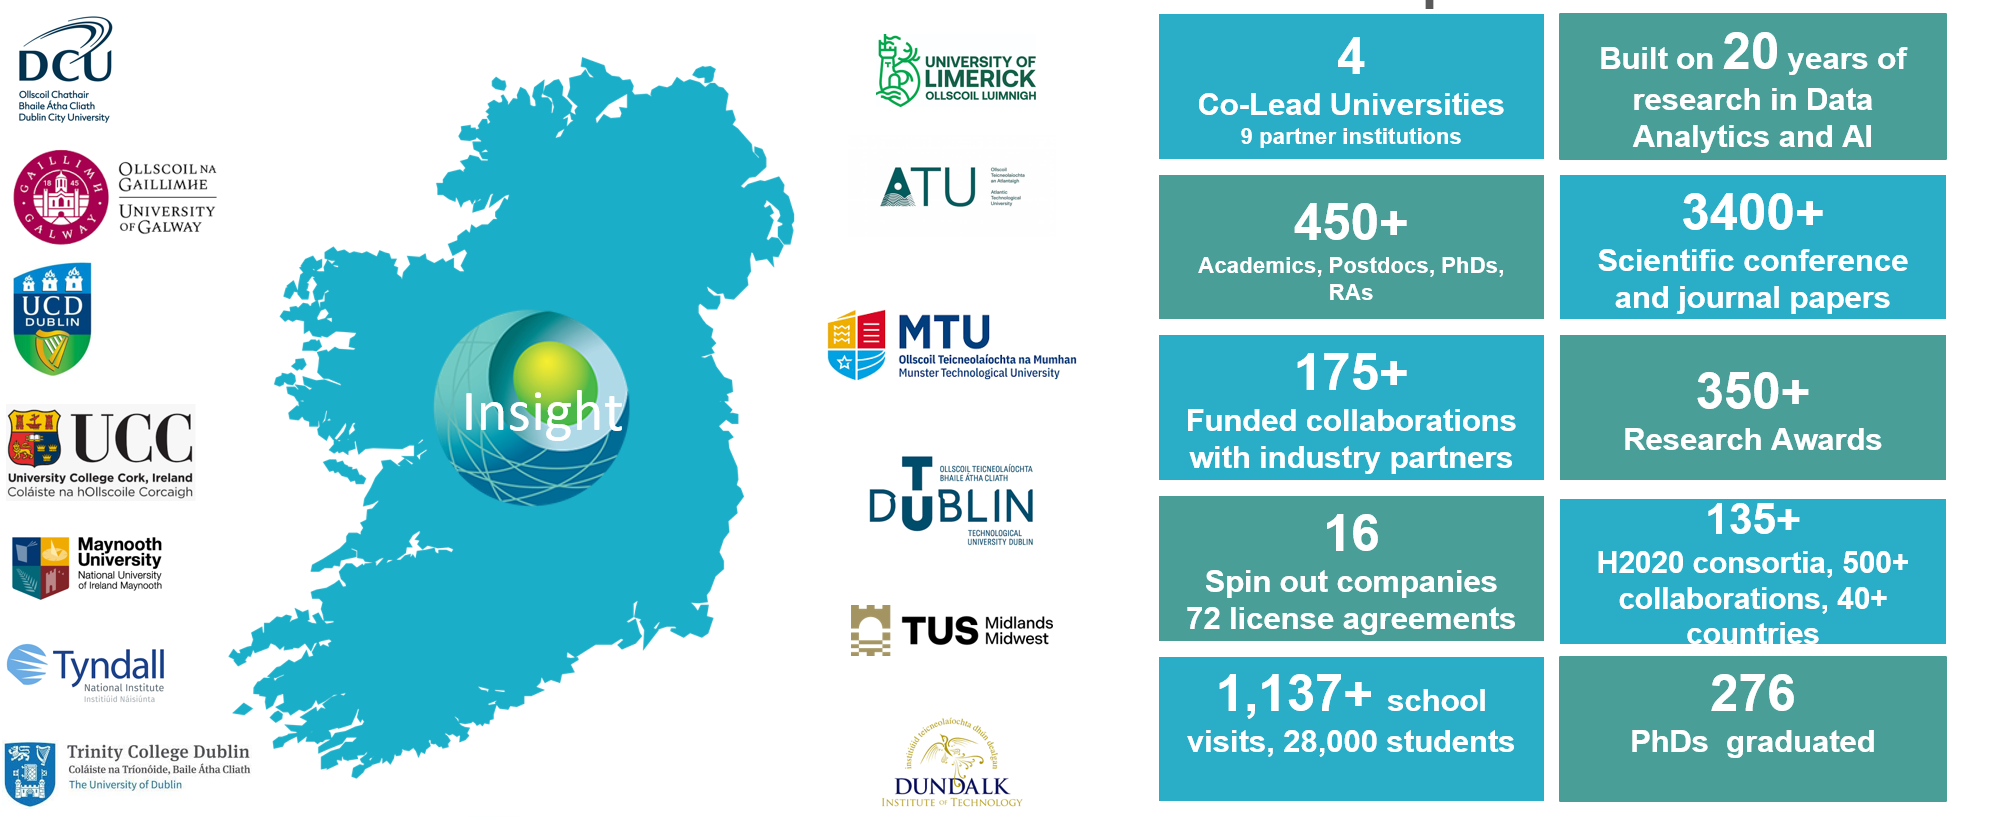
\includegraphics[width=\textwidth]{../summerschool2026/images/onepage}
\end{frame}

\begin{frame}[fragile]
\frametitle{Rinn Artificial Intelligence: Research \& Innovation in Data Science and AI}
\begin{columns}
\begin{column}{0.65\textwidth}
\begin{quotation}
Rinn Artificial Intelligence is designed to serve as a national hub for research and innovation in data science and AI. The programme has two overarching goals: (i) to advance foundational cutting-edge research in Data Science and AI, and (ii) to pursue open, international, and inter- and transdisciplinary research aimed at studying, designing, and implementing strategies to address societal challenges.
\end{quotation}
\end{column}
\begin{column}{0.35\textwidth}

\includegraphics[width=.85\textwidth]{../summerschool2026/images/rinnailogo}
\end{column}
\end{columns}
\end{frame}

\begin{frame}
\frametitle{Background}
\begin{columns}
\begin{column}{0.70\textwidth}
\begin{itemize}
\item Mathematics @ TH Darmstadt
\item 1986-1990 ECRC GmbH, Munich
\item 1990-2000, Technical Director, Cosytec SA, Orsay
\item 2000-2005, Imperial College London, Parc Technologies Ltd
\item 2013-2014, President, Association for Constraint Programming
\item Best Application Paper Awards, CP 2009, CP 2013
\item Program Chair, CP 2020, CPAIOR 2014
\item Distinguished Service Award, ACP
\item Editor in Chief, Constraints, 2026
\end{itemize}
\end{column}
\begin{column}{0.30\textwidth}
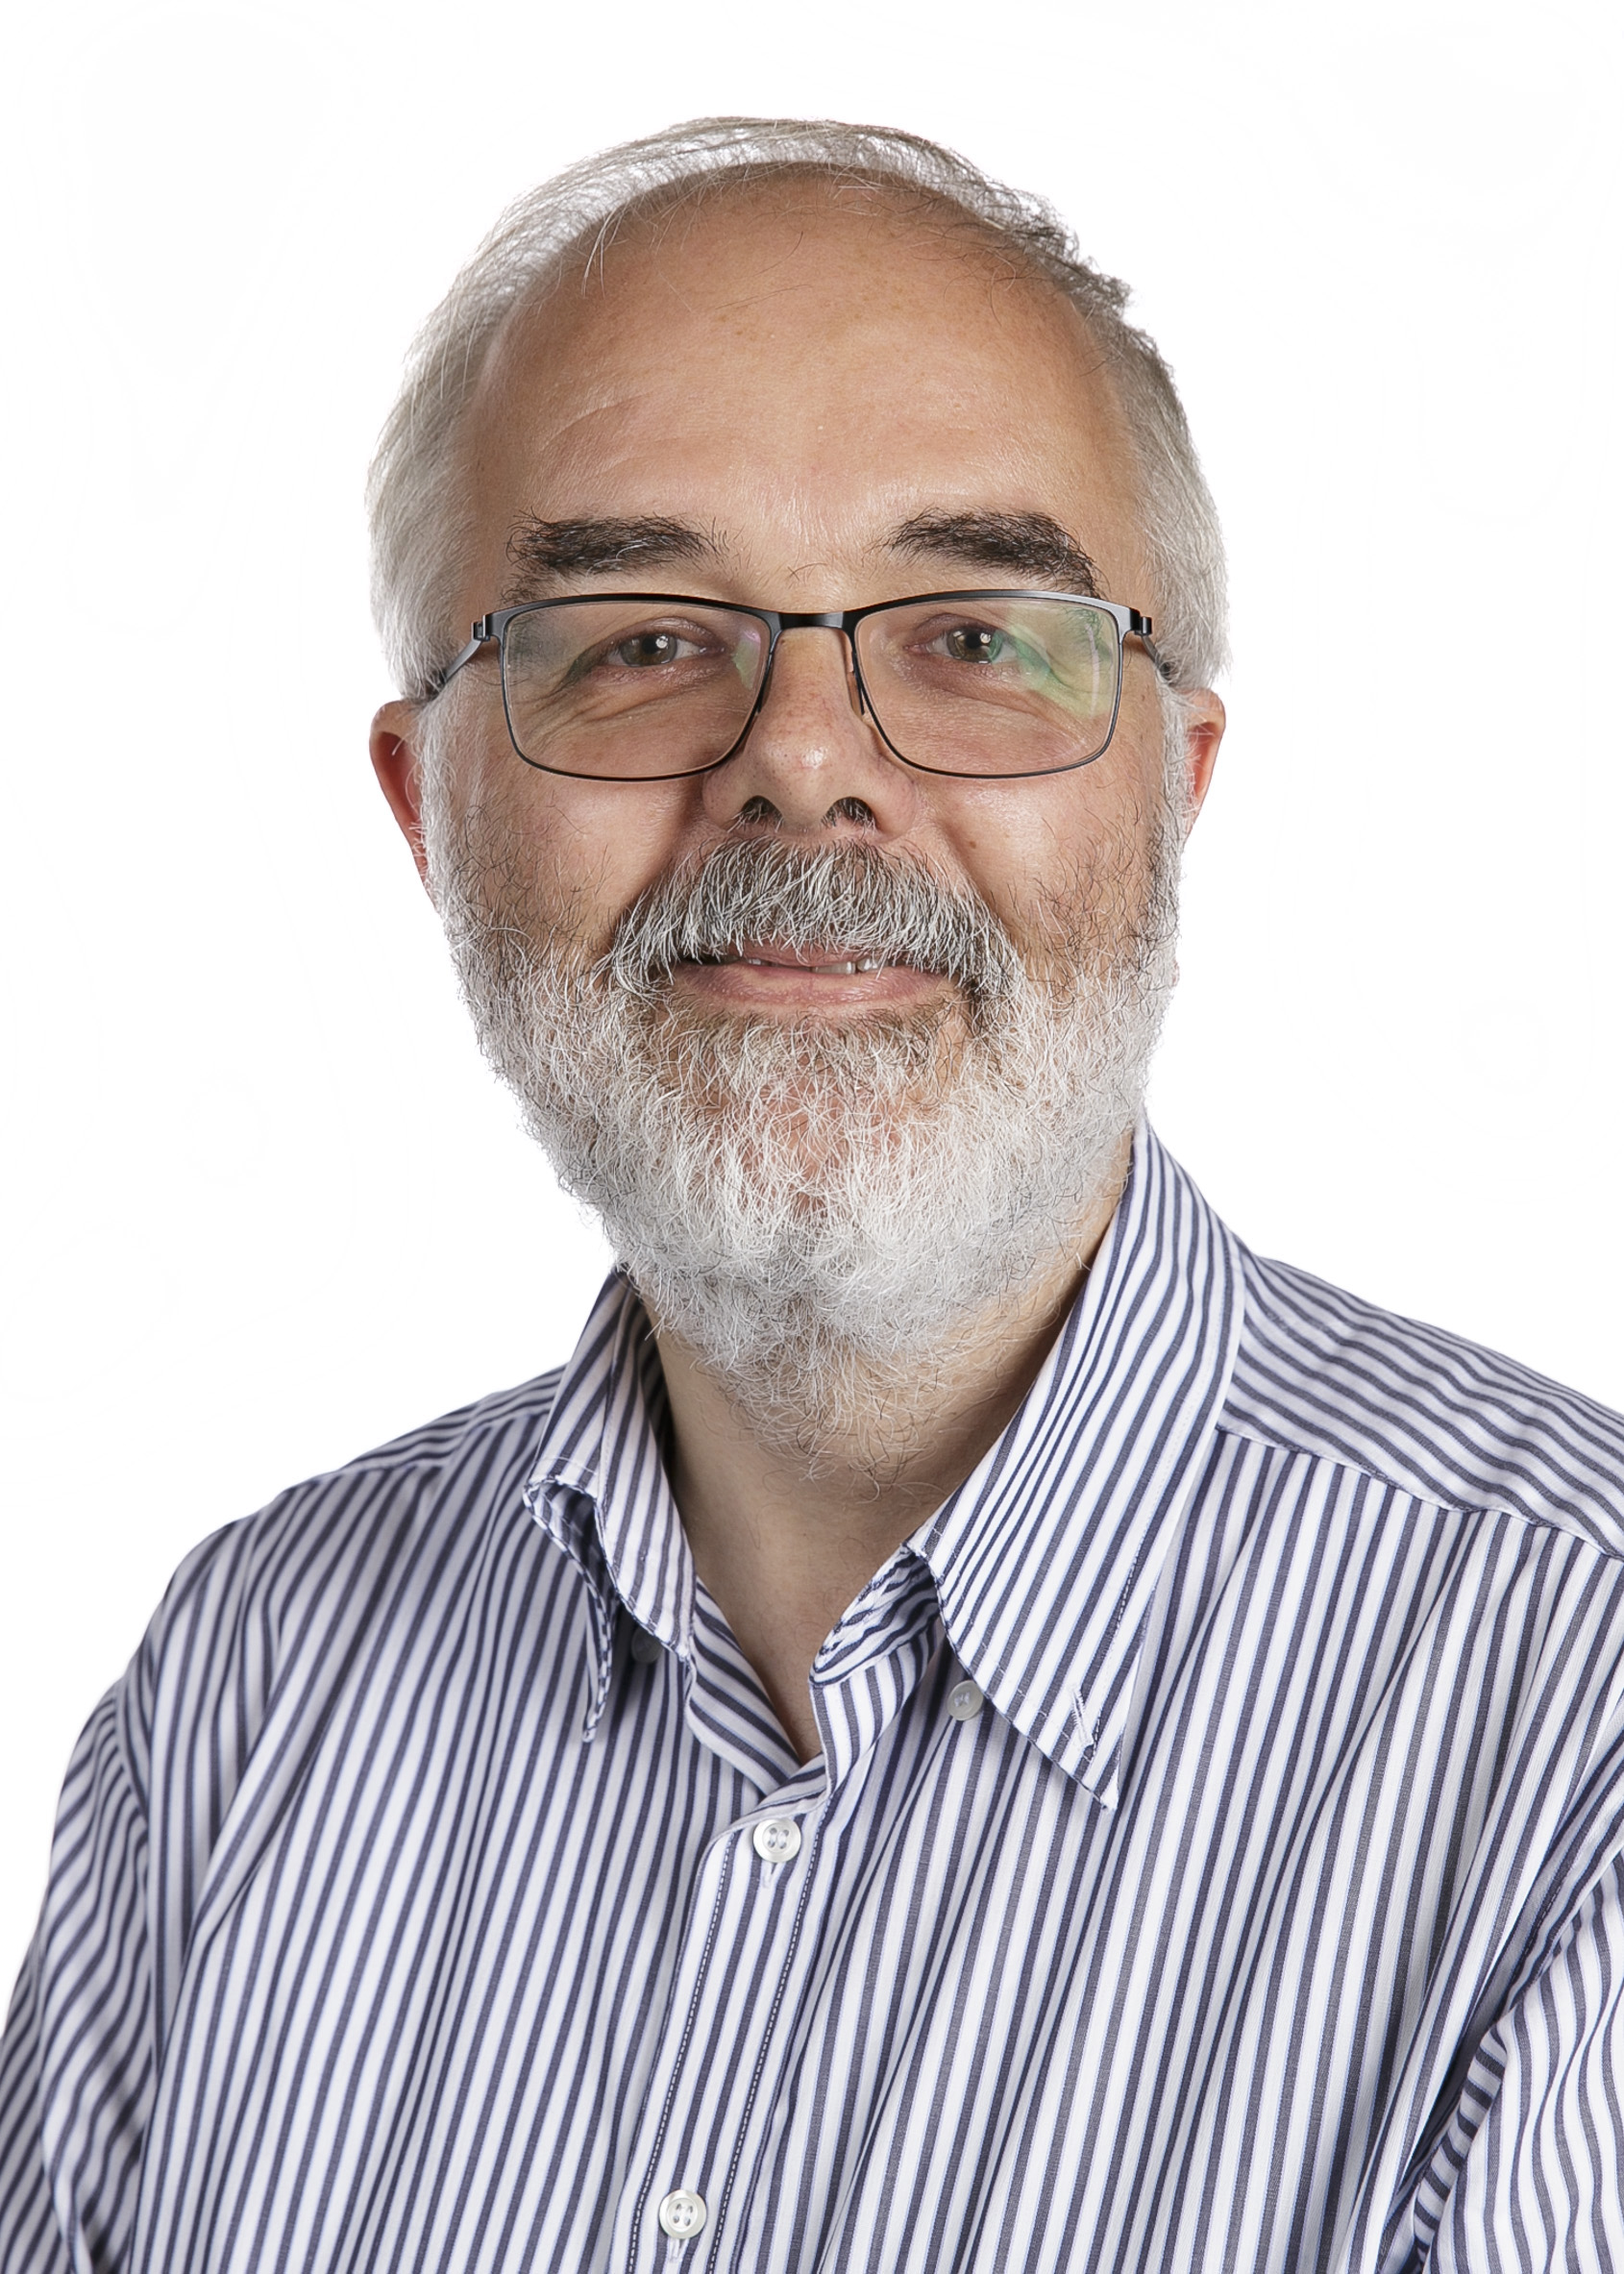
\includegraphics[width=.85\textwidth]{../summerschool2026/images/helmut}
\end{column}
\end{columns}
\end{frame}

\begin{frame}
\frametitle{Applications are important}
\begin{itemize}
\item Provide motivation for basic research
\begin{itemize}
\item Which constraints, methods are needed
\end{itemize}
\item Provide realistic benchmark problems
\begin{itemize}
\item Easy to optimize for pointless results
\end{itemize}
\item Shows that research has potential benefits
\begin{itemize}
\item Much easier to convince funding agencies
\end{itemize}
\item Typically much easier to explain than solver internals
\begin{itemize}
\item Adds motivation, helps with outreach
\end{itemize}
\end{itemize}
\end{frame}

\begin{frame}
\frametitle{Structure of Presentation}
\begin{itemize}
\item Application areas
\item Real-world examples
\begin{itemize}
\item Work in Cork
\end{itemize}
\item Success stories
\begin{itemize}
\item Based on impact
\end{itemize}
\item Methodology
\begin{itemize}
\item How to develop applications, do's and don'ts
\end{itemize}
\item Additional resources
\end{itemize}
\end{frame}

\part{Application Areas for CP}
\frame{\partpage}

\mode<all>{\begin{frame}
\frametitle{Main Application Areas for CP}
\begin{itemize}
\item Scheduling
\item Product Configuration
\item Rostering and Assignment
\item Software/Hardware Design and Testing
\item Transportation
\end{itemize}
\end{frame}

\section{Scheduling}

\begin{frame}
\frametitle{Scheduling Demo}
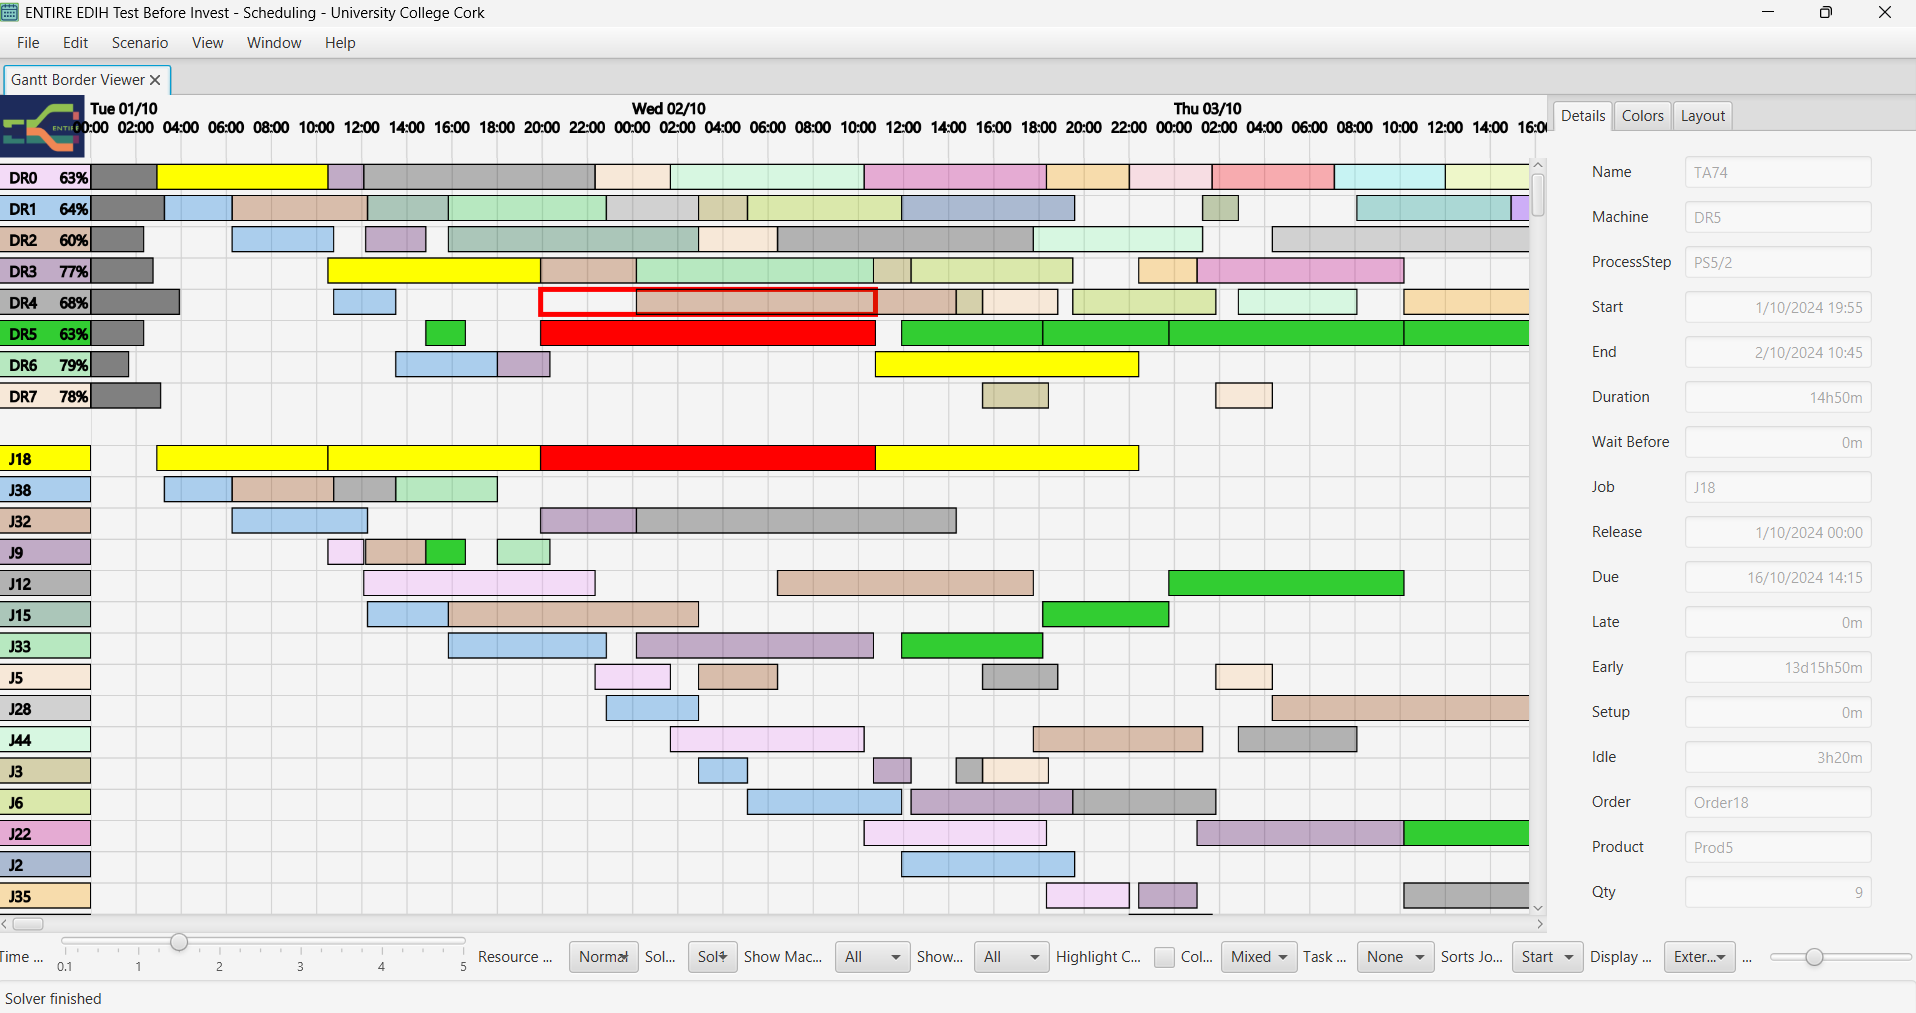
\includegraphics[width=12cm]{images/demoscheduling}
\end{frame}

\begin{frame}
\frametitle{More on Scheduling}
\begin{itemize}
\item Later in this presentation
\item One hour talk in the \href{http://schedulingseminar.com}{Scheduling Seminar} series
\item Video \url{https://www.youtube.com/embed/6fSRT64XE9w?si=B-hcivmO__q9fapD}
\item Slides \url{https://schedulingseminar.com/presentations/schedulingseminar_helmutsimonis.pdf}
\end{itemize}
\end{frame}

\section{Configuration}

\begin{frame}
\frametitle{Product Configuration}
\begin{itemize}
\item Used for semi-custom products
\item Product consist of many different components
\item Many choices for each component type from a catalog
\item Strong constraints between different components
\begin{itemize}
\item Power
\item Bandwidth
\item Space
\item Thermal limits
\end{itemize}
\item Overall objectives: cost, power, space
\end{itemize}
\end{frame}

\begin{frame}
\frametitle{Configuration Example: Railway Signalling (Siemens Austria)}
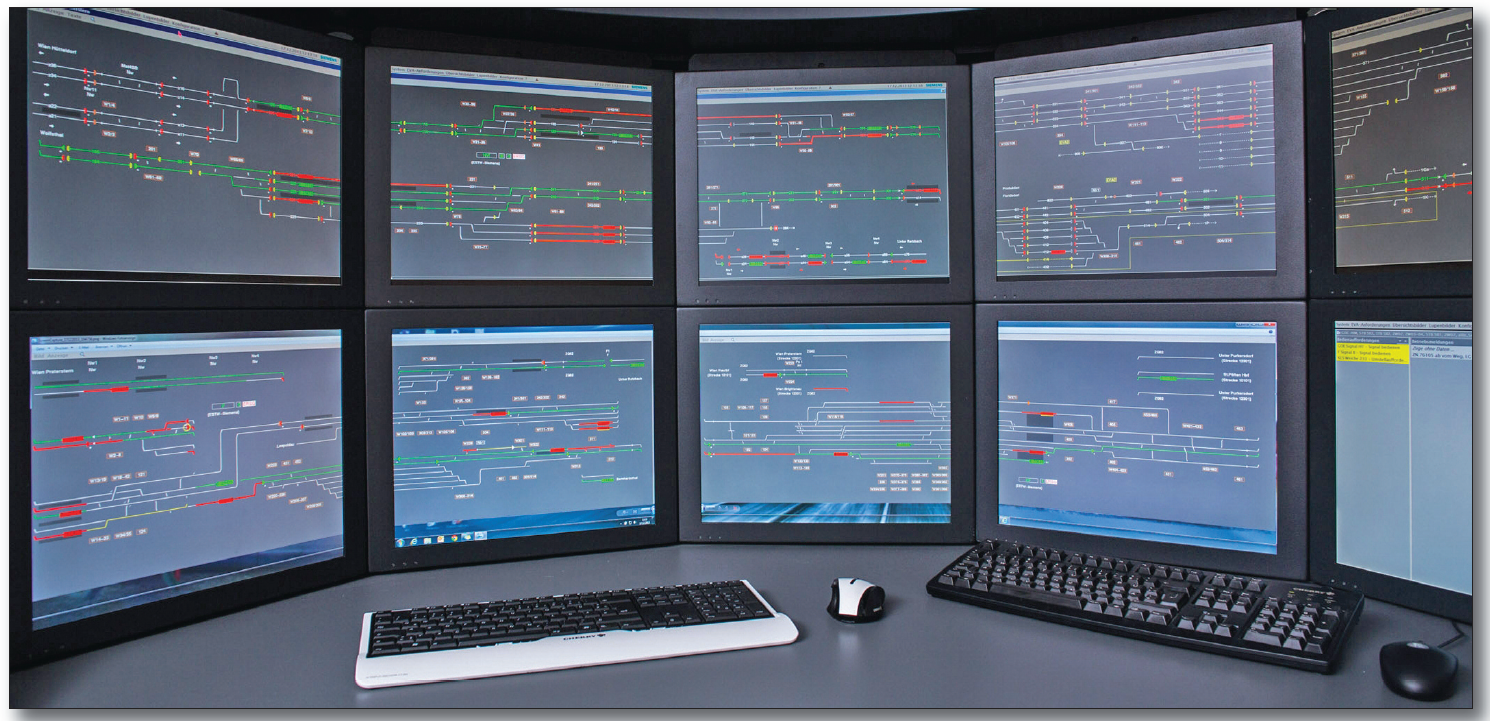
\includegraphics[width=12cm]{images/stellwerkgui}

{\tiny from Falkner  et al, 2016}
\end{frame}

\begin{frame}
\frametitle{Configuration Example: Configurable Hardware (Siemens Austria)}
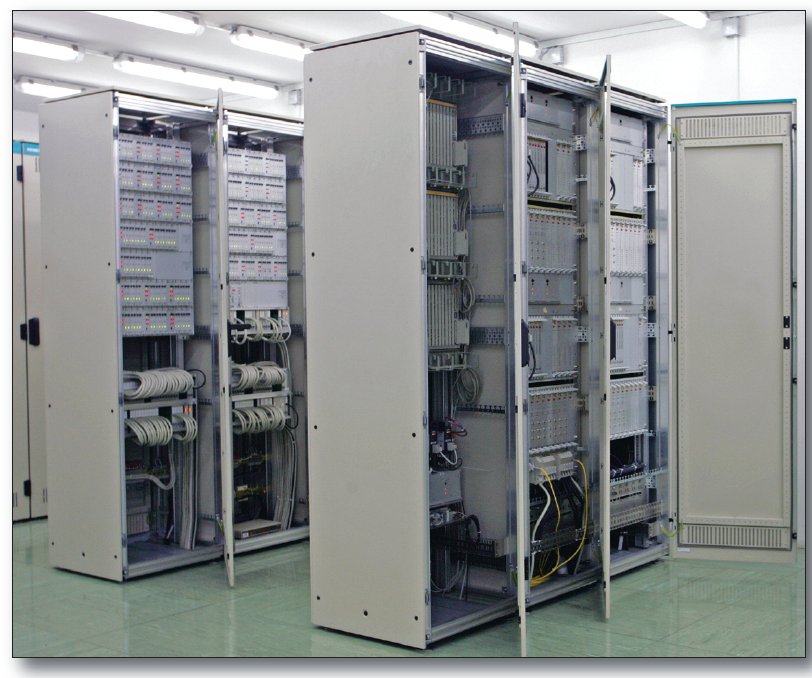
\includegraphics[width=8cm]{images/stellwerkhardware}

{\tiny from Falkner  et al, 2016}
\end{frame}

\begin{frame}
\frametitle{Configuration Modelling}
\begin{itemize}
\item Variables describing alternative component choices
\item Properties of components described by \texttt{table} constraints
\item Linear constraints for global properties
\item \texttt{bin-packing} constraints for rack space
\item \texttt{diffn} constraint for non-overlap in 3D space
\item Multi-objective optimization
\end{itemize}
\end{frame}

\begin{frame}
\frametitle{To learn more}
\begin{itemize}
\item Falkner et al, 2016: Twenty-Five Years of Successful Application of Constraint Technologies at Siemens
\item Erik Cervin-Edin, 2025: Lessons Learnt from Developing \& Maintaining the World's Largest CP Model Using MiniZinc
\item Ulrich Junker, Chapter 24: Configuration, Handbook of Constraint Programming
\end{itemize}
\end{frame}


\section{Rostering}

\begin{frame}
\frametitle{Rostering Demo}
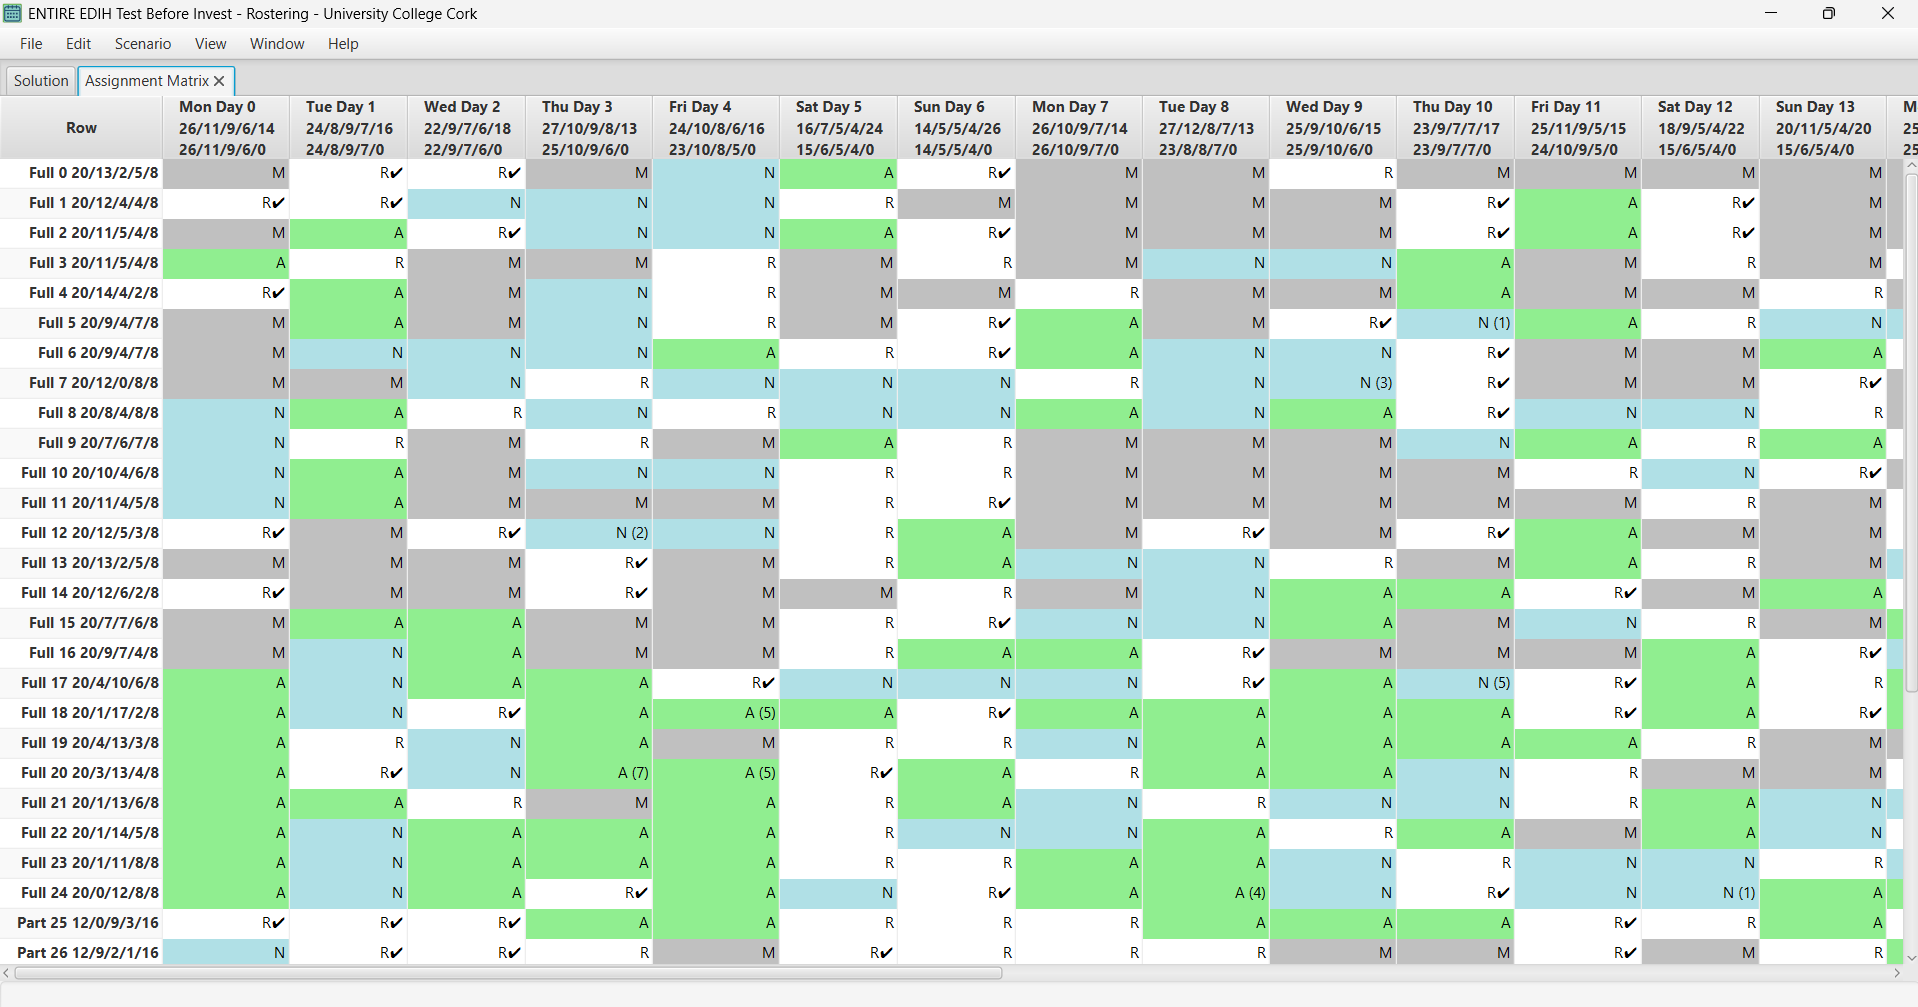
\includegraphics[width=12cm]{images/demorostering}
\end{frame}

\begin{frame}
\frametitle{Rostering}
\begin{itemize}
\item State-of-the-art: Klapperstueck et al, CP 2026: CrewAId: Interactive Optimisation for Human-In-The-Loop Crew Rostering and Rerostering
\item Older: Ernst et al, EJOR 2004: Staff scheduling and rostering: A review of applications, methods and model
\end{itemize}
\end{frame}


\section{Timetabling}

\begin{frame}
\frametitle{Timetabling Demo}
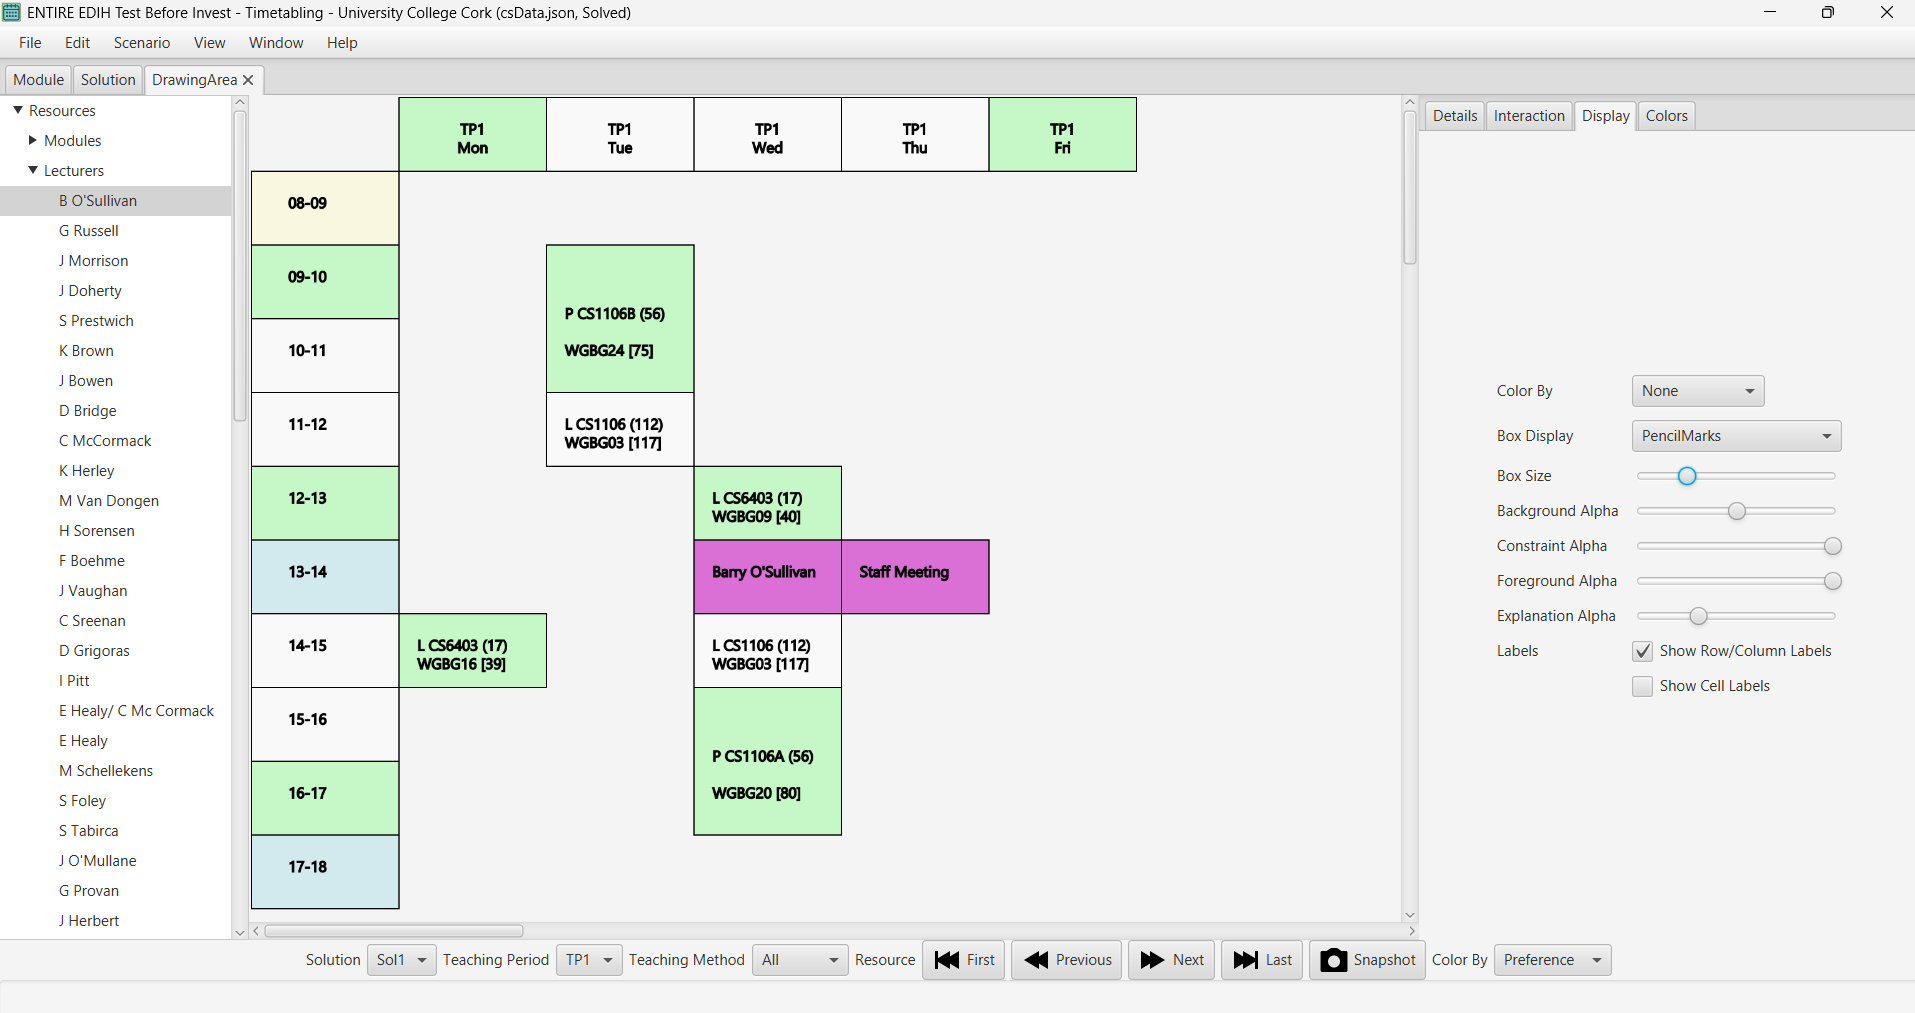
\includegraphics[width=12cm]{images/demotimetabling}
\end{frame}

\begin{frame}
\frametitle{Timetabling}
\begin{itemize}
\item School timetabling
\begin{itemize}
\item Start with Demirovi\`{c}, E., Stuckey, P.J. (2018). \href{https://link.springer.com/chapter/10.1007/978-3-319-93031-2_10}{Constraint Programming for High School Timetabling: A Scheduling-Based Model with Hot Starts}. CPAIOR 2018.
\end{itemize}
\item University timetabling
\begin{itemize}
\item Classic: H.J. Goltz, 1999: University Timetabling using Constraint Logic Programming
\end{itemize}
\item Exam timetabling
\begin{itemize}
\item Good introduction: S. Hamilton, MSc Thesis 2022: Constraint Programming Models For Real-World Examination Scheduling
\end{itemize}
\end{itemize}
\end{frame}

\section{Test/Verification}

\begin{frame}
\frametitle{Test/Verification}
\begin{itemize}
\item Not my area of expertise
\item Specialised CP solvers
\begin{itemize}
\item New domain types, e.g. uint32
\item New constraints, e.g. integer overflow arithmetic
\end{itemize}
\item To learn more: Arnaud Gotlieb video \url{https://www.youtube.com/watch?v=E1Seayx3eXU}
\end{itemize}
\end{frame}

\section{Transportation}

\begin{frame}
\frametitle{Transport Example: TACT}
\begin{itemize}
\item Transporting chickens and turkeys from farms to factory
\begin{itemize}
\item Source of Chicken McNuggets in UK
\end{itemize}
\item Sun Valley Food (Cargill), Hereford, UK
\item Primary objective: Keep factory supplied with birds
\item Multi-resource transport problem
\begin{itemize}
\item Catching teams
\begin{itemize}
\item Drive to farm, catch birds, put in cages, put cages on trucks, go to next farm
\end{itemize}
\item Drivers
\begin{itemize}
\item Drive to farm, load truck with forklift, drive to factory, unload, clean truck, next trip
\end{itemize}
\item Trucks
\begin{itemize}
\item Different vehicle sizes/capacity depends on temperature
\end{itemize}
\end{itemize}

\end{itemize}
\end{frame}

\begin{frame}
\frametitle{Producer/Consumer Constraint for Factory}
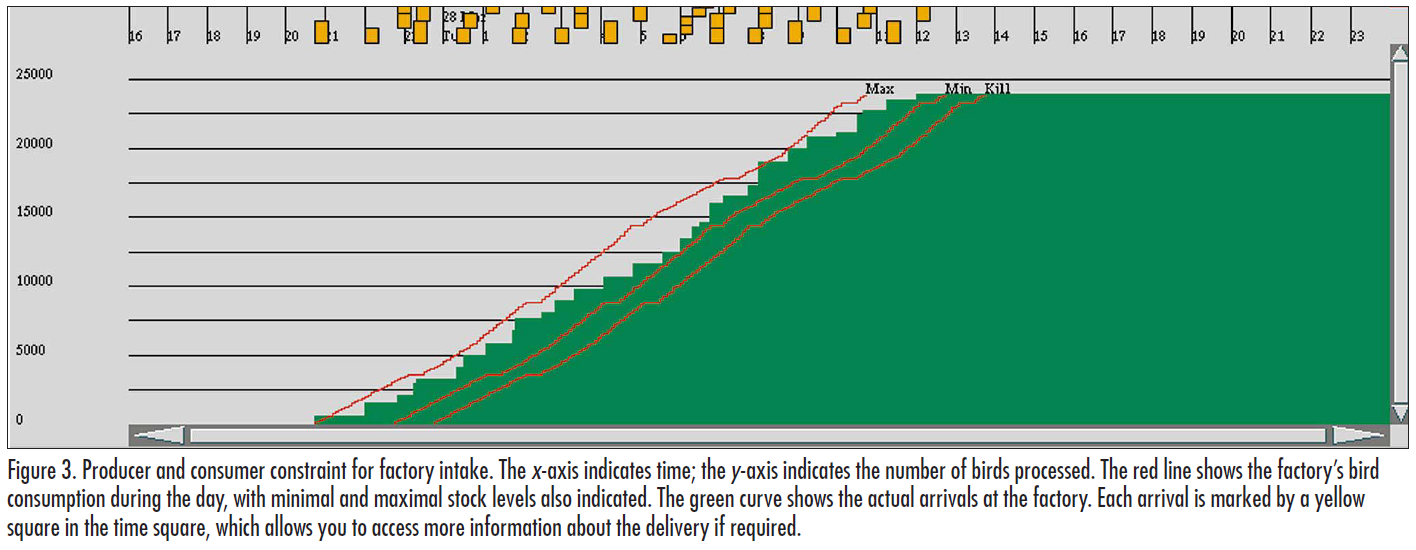
\includegraphics[width=14cm]{../summerschool2026/images/producerconsumer}
\begin{itemize}
\item Do not run factory out of birds!
\item Do not deliver birds too early
\end{itemize}
\end{frame}

\begin{frame}
\frametitle{Order Book}
\begin{columns}
\begin{column}{0.5\textwidth}
\begin{itemize}
\item All trucks/drivers start/end at depot
\item Schedule multiple trips to farms
\begin{itemize}
\item Plan correct number of trips to get all birds from farm
\item Number of trip depends on lorries used
\end{itemize}
\item Transport birds to factory
\item Some transfers between farms
\end{itemize}
\end{column}
\begin{column}{0.5\textwidth}
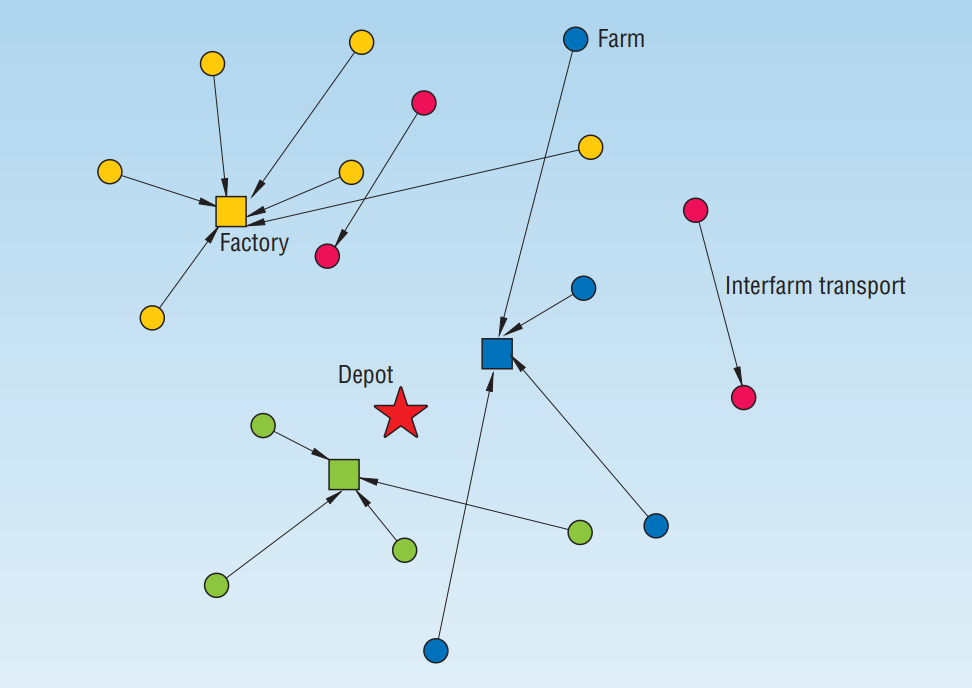
\includegraphics[width=\textwidth]{../summerschool2026/images/orderbook}
\end{column}
\end{columns}
\end{frame}

\begin{frame}
\frametitle{Driver Assignment}
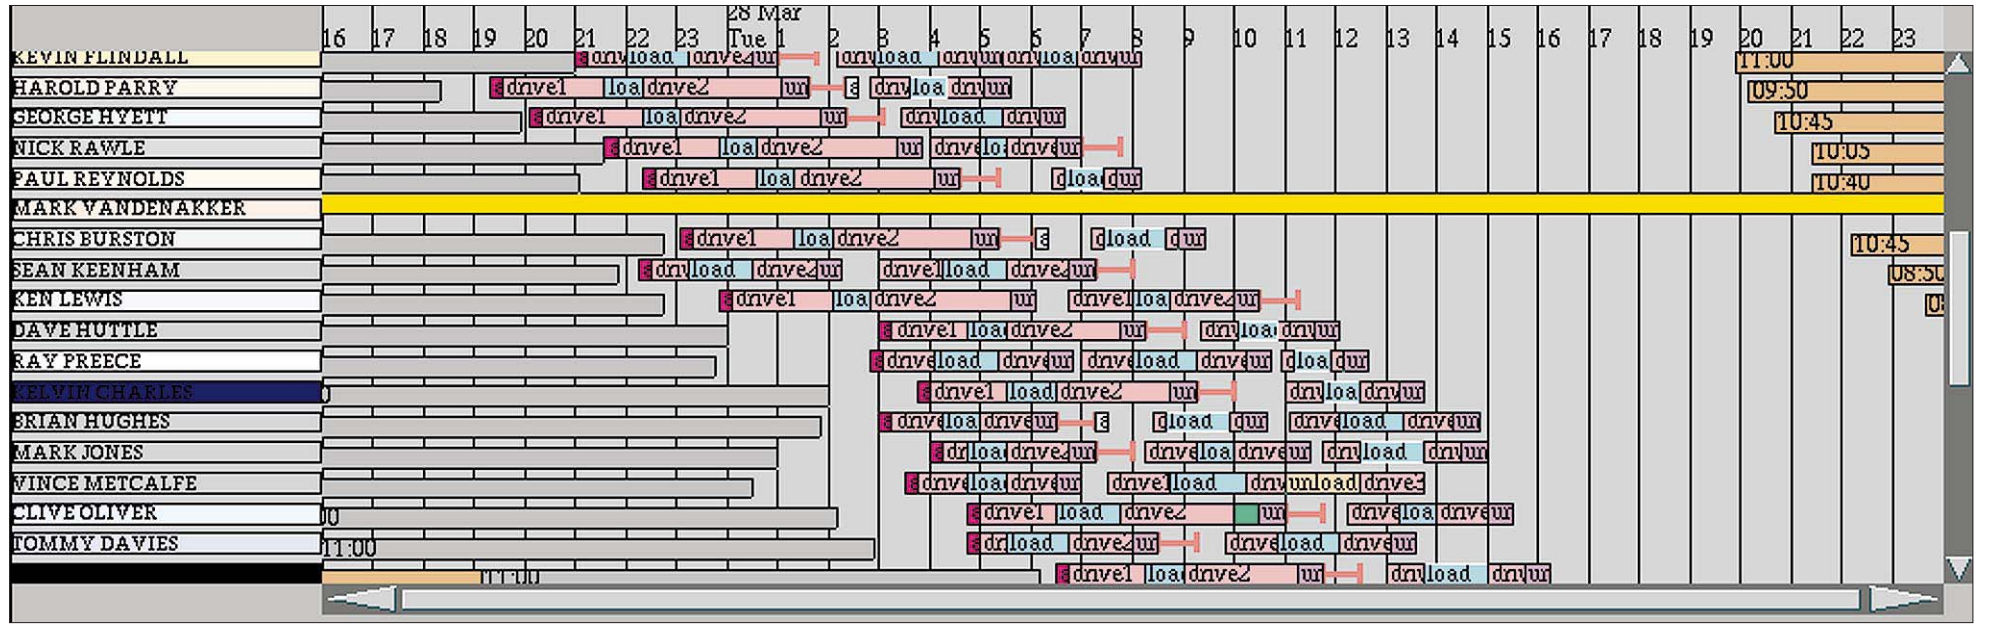
\includegraphics[width=12cm]{../summerschool2026/images/driverassignment}
\begin{itemize}
\item Drivers make 2-4 round trips per day
\item Extra truck/drivers needed for peak demand (cost!)
\item Schedule of one day influences next day (legal rest periods)
\end{itemize}
\end{frame}

\begin{frame}
\frametitle{Truck Assignment}
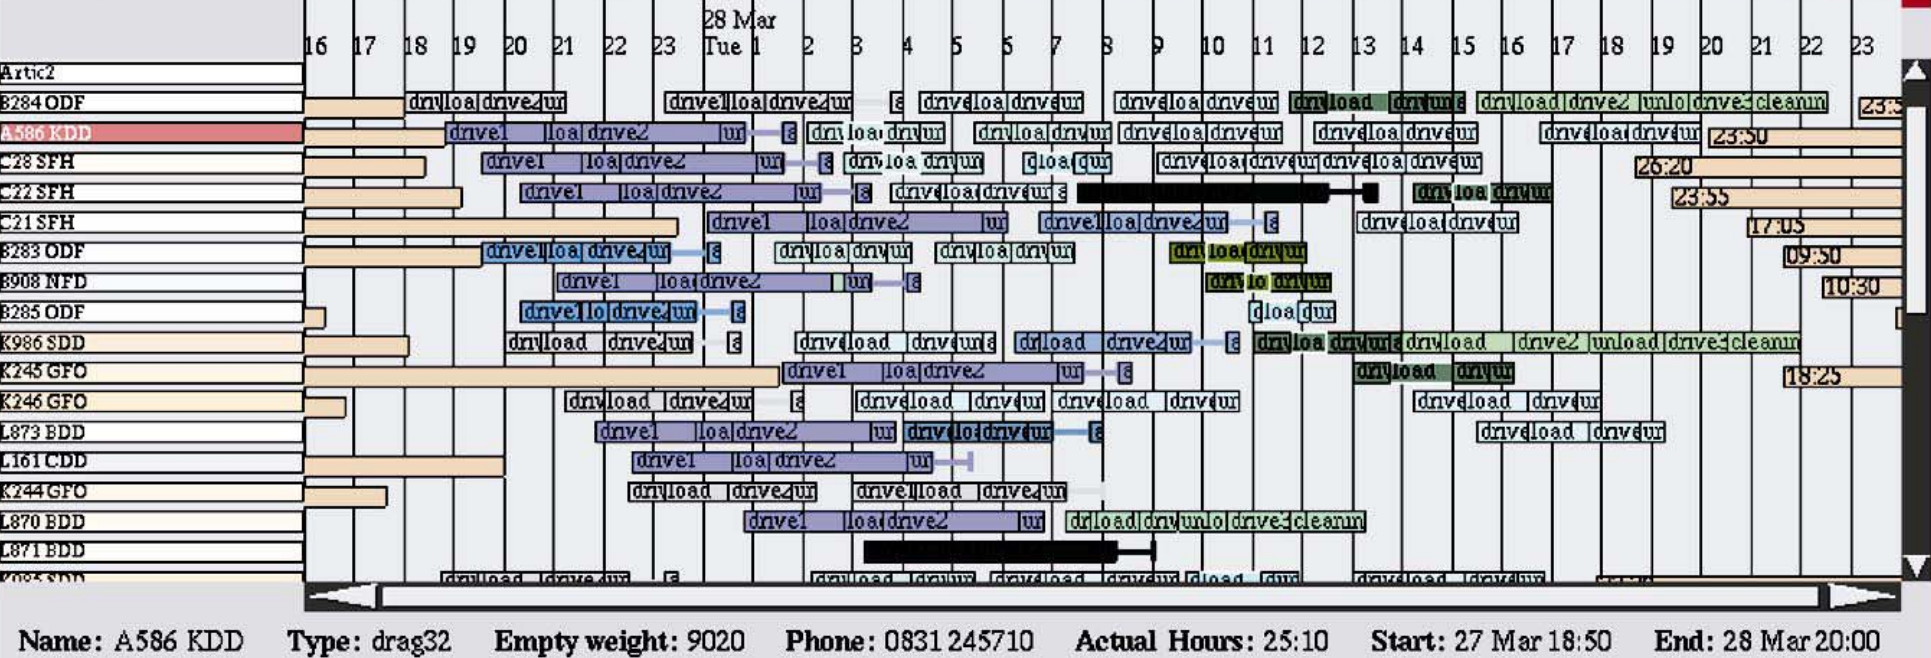
\includegraphics[width=12cm]{../summerschool2026/images/truckassignment}
\begin{itemize}
\item Restrictions of lorry size on certain farms
\item Provide correct transport capacity to get all birds from farms
\item Transport of fork-lifts on truck
\end{itemize}
\end{frame}

\begin{frame}
\frametitle{System}
\begin{itemize}
\item Developed by COSYTEC with CHIP
\item GUI connected to solver and commercial systems
\item Turn-key solution for manager
\item Flexible interactive tool for scheduling expert
\item To learn more: Simonis et al, 2000: Constraint Handling in an Integrated Transportation Problem.
\item More modern solver: Delecluse et al., CP 2022, \href{https://drops.dagstuhl.de/entities/document/10.4230/LIPIcs.CP.2022.19}{Sequence Variables for Routing Problems}

\end{itemize}
\end{frame}

}

\part{Real World Examples}
\frame{\partpage}

\mode<all>{\begin{frame}
\frametitle{More Detailed Example Applications}
\begin{itemize}
\item Flexible Flow-Shop with Transportation Times 
\begin{itemize}
\item J\&J, studies future factory design
\end{itemize}
\item Production Planning and Scheduling
\begin{itemize}
\item Multi-year capacity planning
\item For Siemens Energy, part of ASSISTANT project
\end{itemize}
\item Elevator Maintenance Planning and Scheduling
\begin{itemize}
\item Importance of decomposition
\item Combination with simulation
\end{itemize}
\item Selection of other problem types
\begin{itemize}
\item Only summary slides shown
\end{itemize}
\end{itemize}
\end{frame}


\mode<all>{\input{../summerschool2026/jj}}

\mode<all>{\input{../summerschool2026/siemensenergy}}

\mode<all>{\input{../summerschool2026/fieldservice}}

\section{Other Applications}

\begin{frame}
\frametitle{Other Noteworthy Applications}
\begin{itemize}
\item NVD LoadBuilder
\item Boliden Tara Mines Dewatering
\item Dental School Timetabling
\item Irish Naval Service Rostering
\item Data Centre Load Consolidation
\item Scheduling with Time Variable Energy Prices
\item Characterizing EDF Power Plants with Timeseries Constraints
\item Optical Network Design
\item Supplier Selection Problem
\item Optimizing UCC's CHP Plant Operation
\item CP Conference Paper Assignment Tool
\end{itemize}
\end{frame}

\begin{frame}
\frametitle{NVD LoadBuilder}
\begin{textblock*}{5cm}(9cm,-1cm)
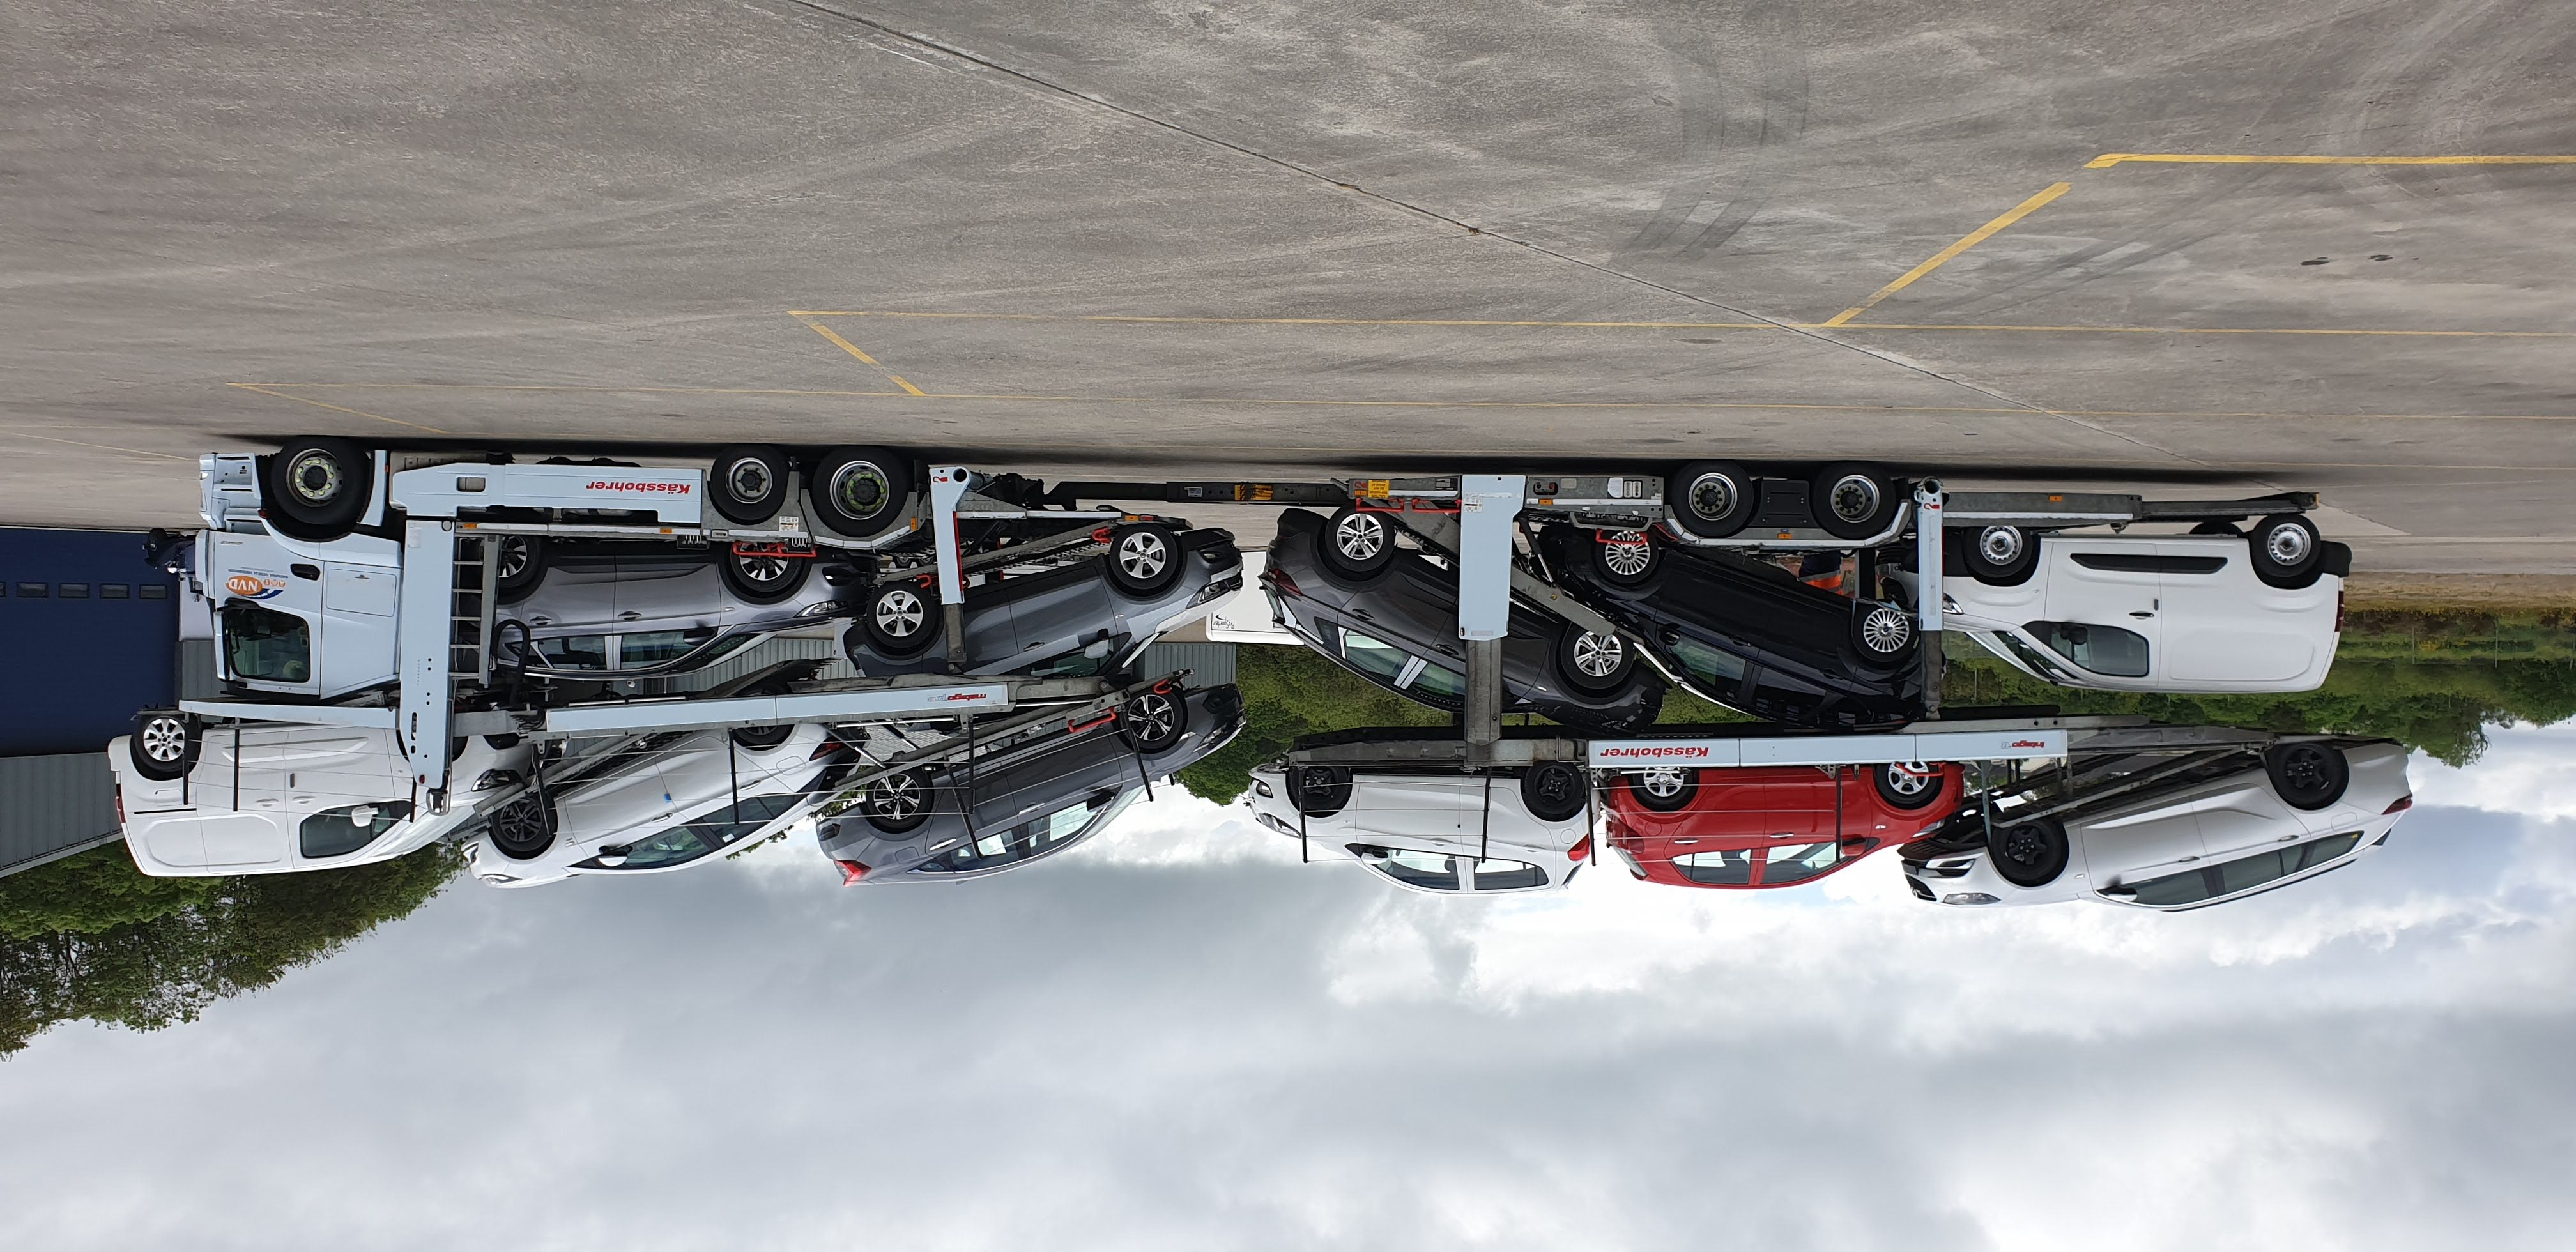
\includegraphics[width=5cm,angle=180]{images/metagointago}
\end{textblock*}

\begin{columns}[b]
\begin{column}{0.5\textwidth}
\begin{itemize}
\item Real-World Problem
\begin{itemize}
\item Deliver cars/vans from factory/ports to dealers
\item Group cars into loads for joint delivery
\item Using specialized transporters with complex configurations
\item Balance distance travelled, utilization of fleet, priority of orders
\end{itemize}
\item Status
\begin{itemize}
\item Operational at customer starting in 2020
\item Start-up company CMC to further develop tool
\end{itemize}
\end{itemize}
\end{column}
\begin{column}{0.5\textwidth}
\begin{itemize}
\item Research Challenges
\begin{itemize}
\item Vehicle routing problem with complex capacity constraints
\item Decide which cars to deliver today
\item What impact does this have tomorrow
\item Explaining solutions to end-user
\end{itemize}
\item Solution Approach
\begin{itemize}
\item Decomposition
\item MIP, Constraint Programming, Local Search, Data Analytics
\end{itemize}
\end{itemize}
\end{column}
\end{columns}
\end{frame}

\begin{frame}
\frametitle{Boliden Tara Mines Dewatering}
\begin{textblock*}{4cm}(9cm,-1cm)
%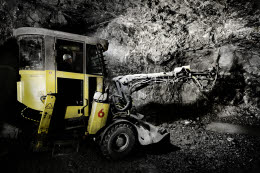
\includegraphics[width=4cm]{images/bolidentara}
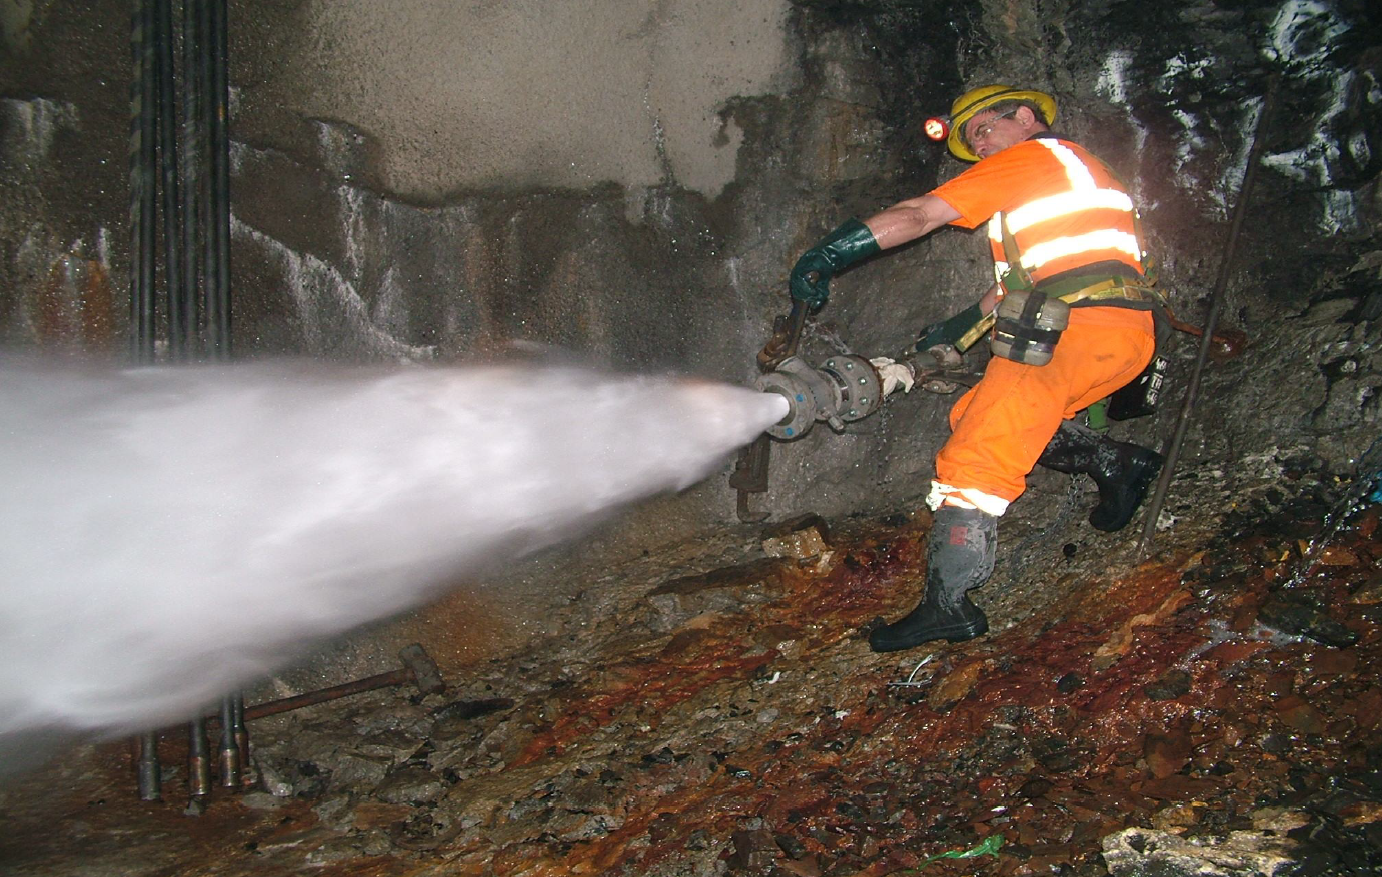
\includegraphics[width=4cm]{images/waterflow}
\end{textblock*}
\vspace{2cm}
\begin{columns}[b]
\begin{column}{0.5\textwidth}
\begin{itemize}
\item Real-World Problem
\begin{itemize}
\item When/how to pump water out of mine
\item Multiple pumps, reservoirs
\item Electricity cost major cost factor
\item Safe operation of mine paramount
\end{itemize}
\item Status
\begin{itemize}
\item Student-led project with DCU
\item Paper at AAAI 2016
\item Major flooding event in 2021
\end{itemize}
\end{itemize}
\end{column}
\begin{column}{0.5\textwidth}
\begin{itemize}
\item Research Challenges
\begin{itemize}
\item Scheduling with uncertain energy prices (real-time tariff)
\item Uncertain water ingress depends on operations
\item Capacity (min/max) constraints for storage 
\end{itemize}
\item Solution Approach
\begin{itemize}
\item Electricity price prediction
\item Optimization
\end{itemize}
\end{itemize}
\end{column}
\end{columns}
\end{frame}

\begin{frame}
\frametitle{Dental School Timetabling}
\begin{textblock*}{6cm}(8cm,-1cm)
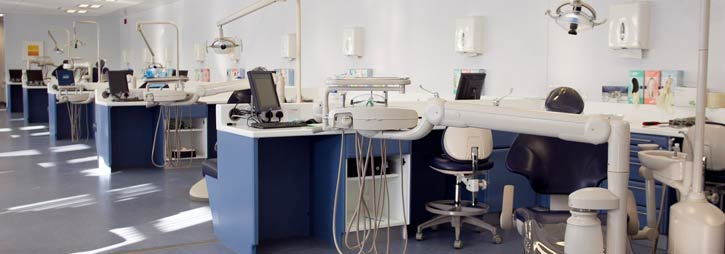
\includegraphics[width=6cm]{images/OrthoClinic}
\end{textblock*}
\begin{columns}[b]
\begin{column}{0.5\textwidth}
\begin{itemize}
\item Real-World Problem
\begin{itemize}
\item Change time table during period of teaching capacity increase
\item Previous schedule no longer feasible
\item Multiple courses share same lab space (dental chairs) at the same time
\item Hard capacity limits on available resources and time slots
\end{itemize}
\item Status
\begin{itemize}
\item Used by dental school during transition period
\item Paper in IAAI 2013, AI Mag 2014
\end{itemize}
\end{itemize}
\end{column}
\begin{column}{0.5\textwidth}
\begin{itemize}
\item Research Challenges
\begin{itemize}
\item Very different from standard timetabling problem
\item Hard/soft capacity constraints
\item Tool cleaning setup time constraints
\end{itemize}
\item Solution Approach
\begin{itemize}
\item Optimization
\item Flexible prioritization of constraints
\end{itemize}
\end{itemize}
\end{column}
\end{columns}
\end{frame}

\begin{frame}
\frametitle{Irish Naval Service Yearly Rostering}
\begin{textblock*}{4cm}(9cm,-1cm)
%
\includegraphics[width=2.5cm]{images/Irish_Naval_Service}
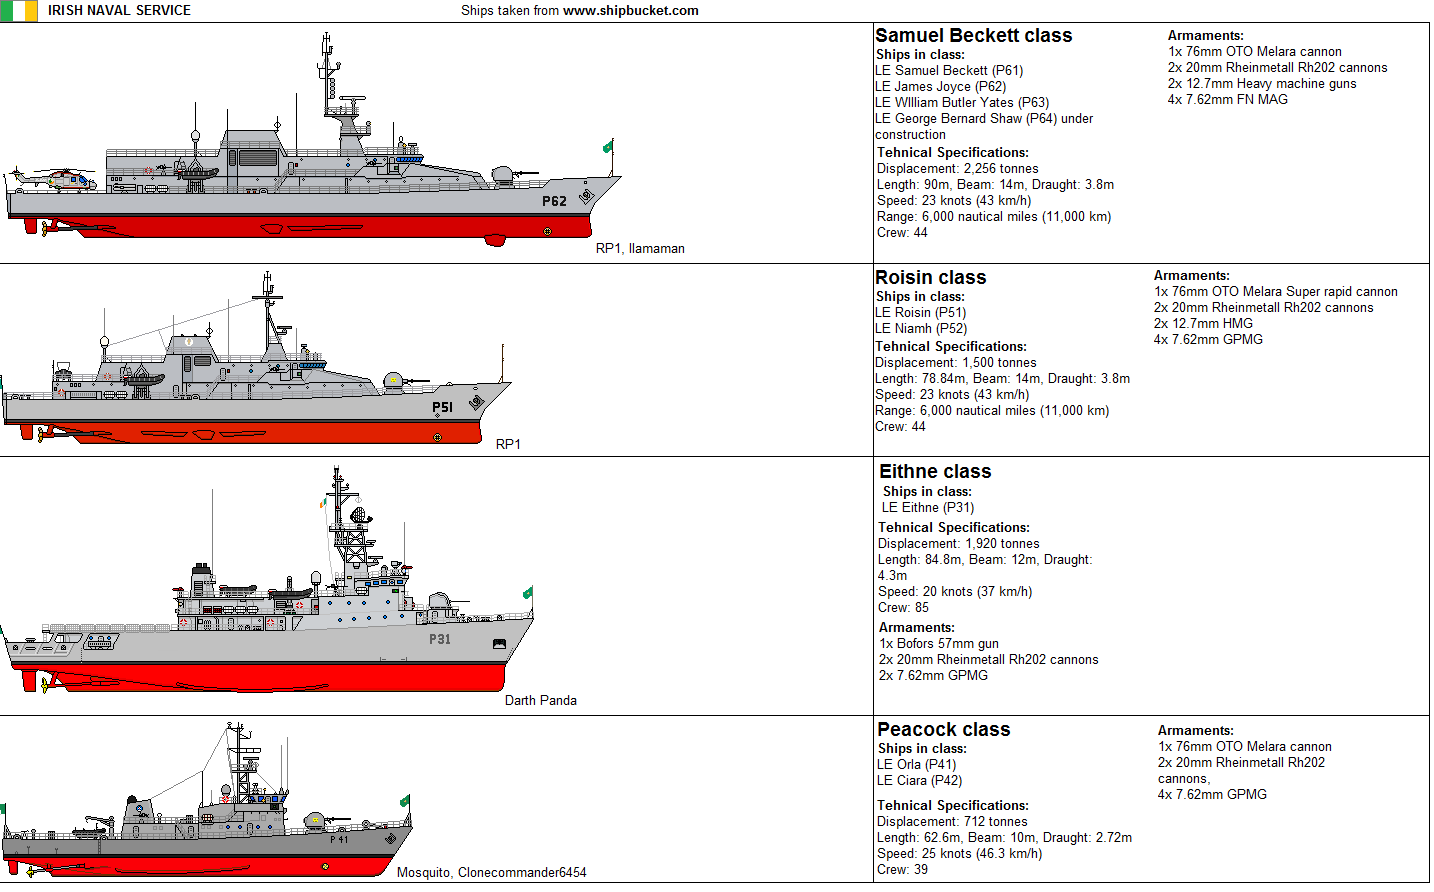
\includegraphics[width=4cm]{images/irish_naval_service_by_zagoreni010_dbaxsq7}
\end{textblock*}
\vspace{1cm}

\begin{columns}[b]
\begin{column}{0.5\textwidth}
\begin{itemize}
\item Real-World Problem
\begin{itemize}
\item Decide which ships are performing which type of duty over the year
\item Budget limitations on total time at sea
\item Fair share of work across fleet
\item Fixed maintenance periods for certain ships
\item Special events (flotilla exercises, detached duty) 
\end{itemize}
\item Status
\begin{itemize}
\item Prototype results produced for service
\end{itemize}
\end{itemize}
\end{column}
\begin{column}{0.5\textwidth}
\begin{itemize}
\item Research Challenges
\begin{itemize}
\item Finding the best tool and model for problem
\item Balanced assignment under budget constraints
\item Provide consistent force levels over whole year
\item Fair assignment of work/rest days across fleet
\end{itemize}
\item Solution Approach
\begin{itemize}
\item Optimization
\end{itemize}
\end{itemize}
\end{column}
\end{columns}
\end{frame}

\begin{frame}
\frametitle{Data Centre Load Consolidation}
\begin{textblock*}{7cm}(8cm,-1cm)
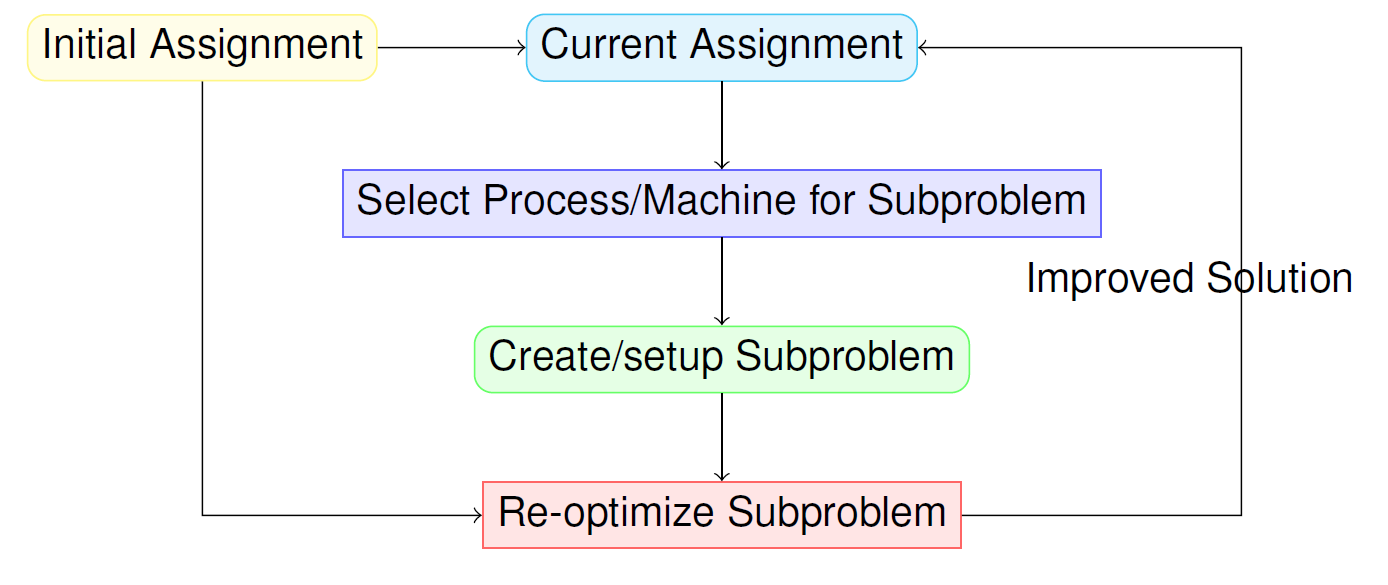
\includegraphics[width=7cm]{images/lnsdesign}
\end{textblock*}
\vspace{1cm}
\begin{columns}[b]
\begin{column}{0.5\textwidth}
\begin{itemize}
\item Real-World Problem
\begin{itemize}
\item Move virtual machines between servers in a data centre
\item Balance/concentrate workload on multiple resource types
\item Extend to multiple data centres across world 
\end{itemize}
\item Status
\begin{itemize}
\item 2nd place in Google Roadef/Euro Challenge 2012
\item Multiple papers
\end{itemize}
\end{itemize}
\end{column}
\begin{column}{0.5\textwidth}
\begin{itemize}
\item Research Challenges
\begin{itemize}
\item Reassignment problem
\item Multi-bin packing constraints
\item Large neighbourhood search to deal with problem size 
\end{itemize}
\item Solution Approach
\begin{itemize}
\item Optimization
\item New tools/propagators
\end{itemize}
\end{itemize}
\end{column}
\end{columns}
\end{frame}

\begin{frame}
\frametitle{Scheduling with Time Variable Energy Prices}
\begin{textblock*}{3cm}(11cm,-1cm)
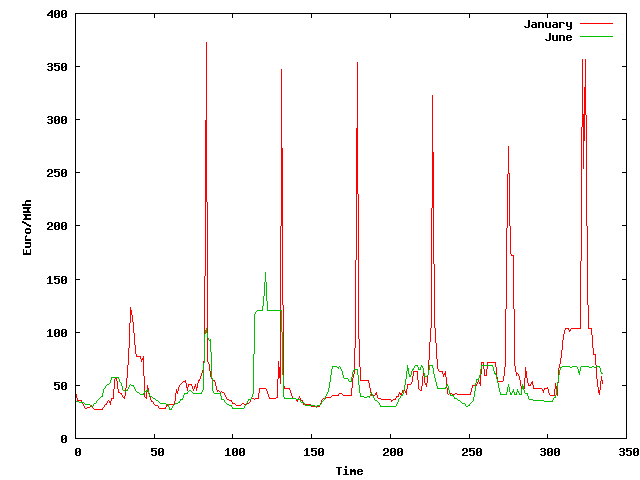
\includegraphics[width=3cm]{images/price}
\end{textblock*}
\vspace{0.8cm}
\begin{columns}[b]
\begin{column}{0.5\textwidth}
\begin{itemize}
\item Real-World Problem
\begin{itemize}
\item How do time-variable electricity prices affect scheduling of use
\item Uncertainty of prices, sudden peak prices common in Ireland
\item In most cases, we have to commit to production before price is known
\item Deal with risk/possible rewards
\end{itemize}
\item Status
\begin{itemize}
\item Multiple papers 
\item Continued work on price prediction with industry
\end{itemize}
\end{itemize}
\end{column}
\begin{column}{0.5\textwidth}
\begin{itemize}
\item Research Challenges
\begin{itemize}
\item Can we use time variable electricity prices to our advantage?
\item Which properties should a price prediction model have to help with scheduling?
\item Can we tune price prediction for the use case it is intended for?
\end{itemize}
\item Solution Approach
\begin{itemize}
\item Machine Learning
\item Optimization
\end{itemize}
\end{itemize}
\end{column}
\end{columns}
\end{frame}

\begin{frame}
\frametitle{Characterizing EDF Power Plants}
\begin{textblock*}{3cm}(10cm,-1cm)
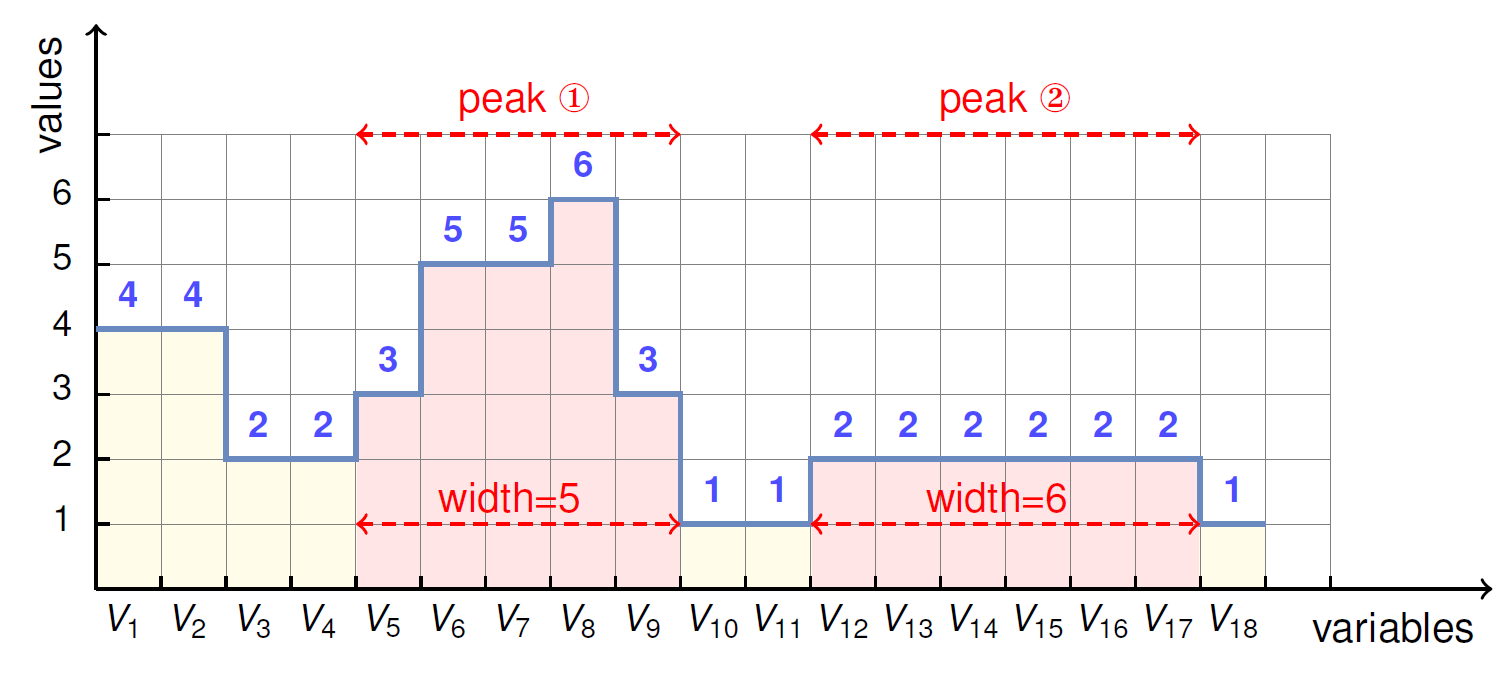
\includegraphics[width=3cm]{images/minwidthpeak}
\end{textblock*}

\begin{columns}[b]
\begin{column}{0.5\textwidth}
\begin{itemize}
\item Real-World Problem
\begin{itemize}
\item Unit Commitment Model for electricity supply
\item Decide which units to run when to satisfy demand/minimize cost
\item Change of production for different units is limited over time
\item Very error-prone integration into global model
\end{itemize}
\item Status
\begin{itemize}
\item Joint work with IMT-Atlantique, EDF Research
\item Series of papers on time-series constraints, Volume II of Global Constraint Catalog
\end{itemize}
\end{itemize}
\end{column}
\begin{column}{0.5\textwidth}
\begin{itemize}
\item Research Challenges
\begin{itemize}
\item Can we characterize the production limits of power plants as time-series constraints?
\item Learn constraints from historical data (planned/actual)
\item Create model of individual plants to describe their capabilities
\item Find redundant constraints to overcome limits of propagation  
%\item Integrate into MIP unit commitment model
\end{itemize}
\item Solution Approach
\begin{itemize}
\item Machine Learning
\item Automata constraints
\item Generated code for propagators
\end{itemize}
\end{itemize}
\end{column}
\end{columns}
\end{frame}

\begin{frame}
\frametitle{Optical Network Design}
\begin{textblock*}{6cm}(8cm,-1cm)
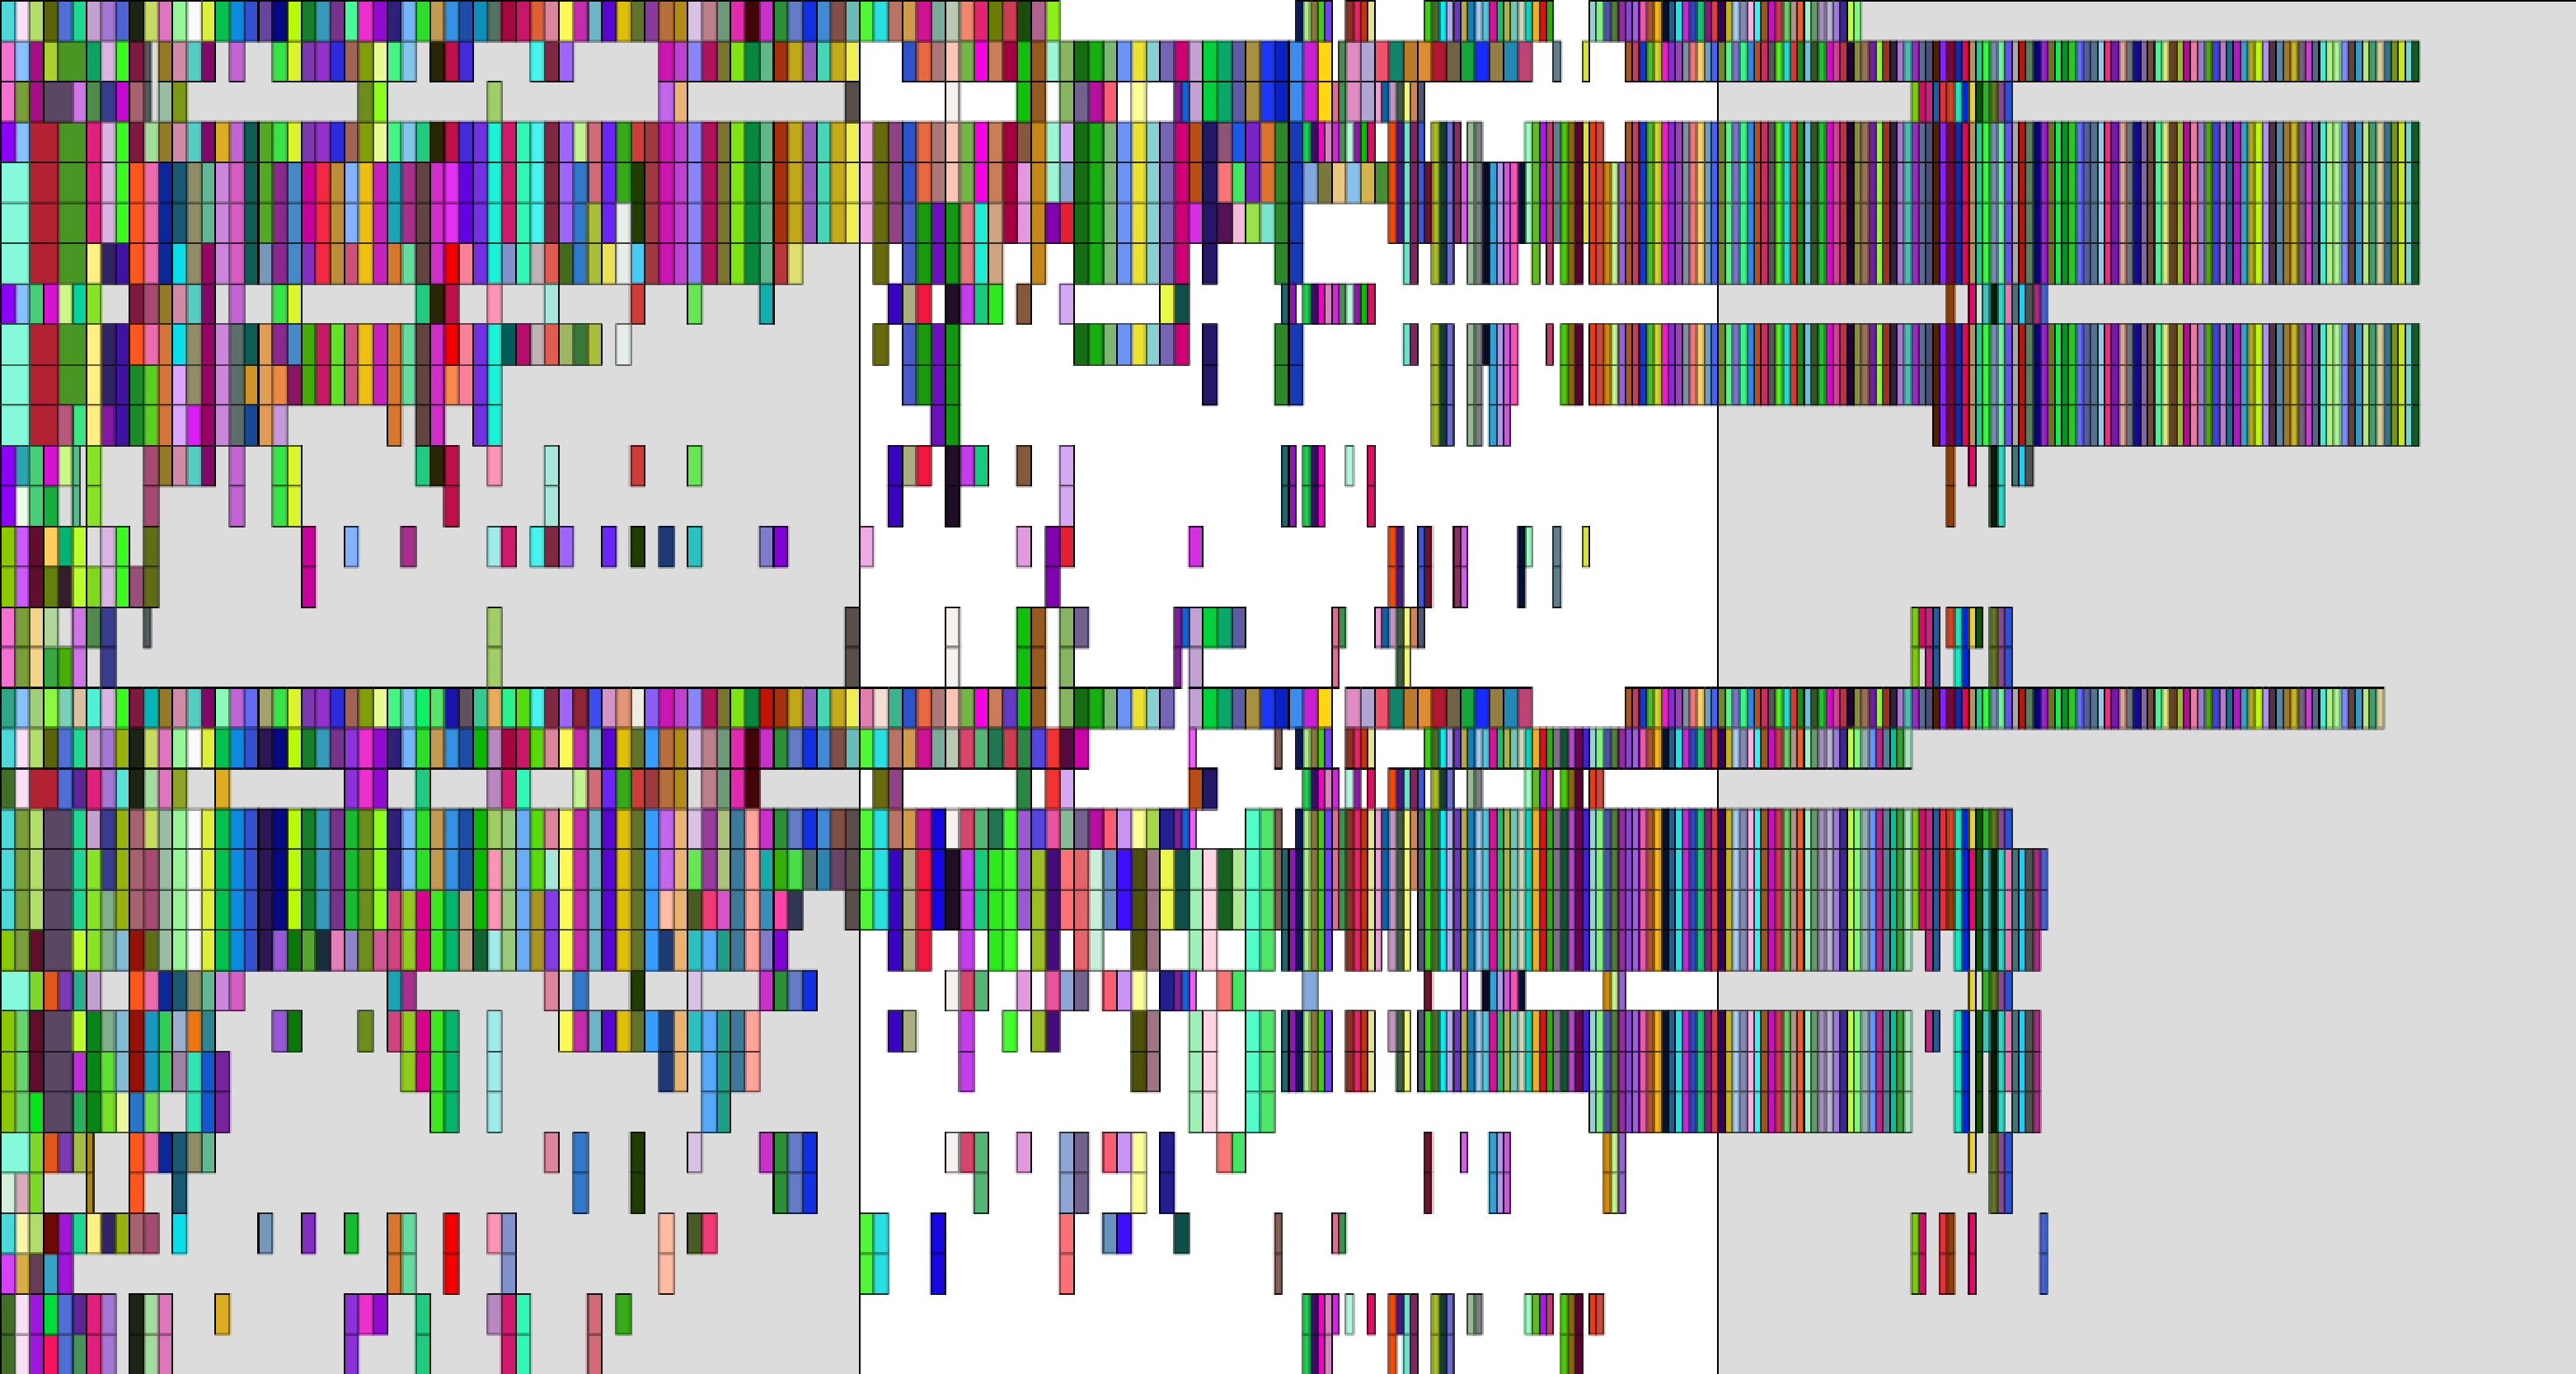
\includegraphics[width=6cm]{images/Ireland18}
\end{textblock*}
\vspace{1cm}
\begin{columns}[b]
\begin{column}{0.5\textwidth}
\begin{itemize}
\item Real-World Problem
\begin{itemize}
\item Core optical network design 
\item Different from traditional IP network design
\item Define paths from source to sink
\item Use multiple frequency (light) bands over same fibre
\end{itemize}
\item Status
\begin{itemize}
\item Paper ICTAI 2014
\end{itemize}
\end{itemize}
\end{column}
\begin{column}{0.5\textwidth}
\begin{itemize}
\item Research Challenges
\begin{itemize}
\item Modelling Choices
\item Amount of propagation achieved
\item Scalability of methods
\end{itemize}
\item Solution Approach
\begin{itemize}
\item Global Constraints
\end{itemize}
\end{itemize}
\end{column}
\end{columns}
\end{frame}

\begin{frame}
\frametitle{Supplier Selection Problem}
\begin{textblock*}{9cm}(6cm,-1cm)
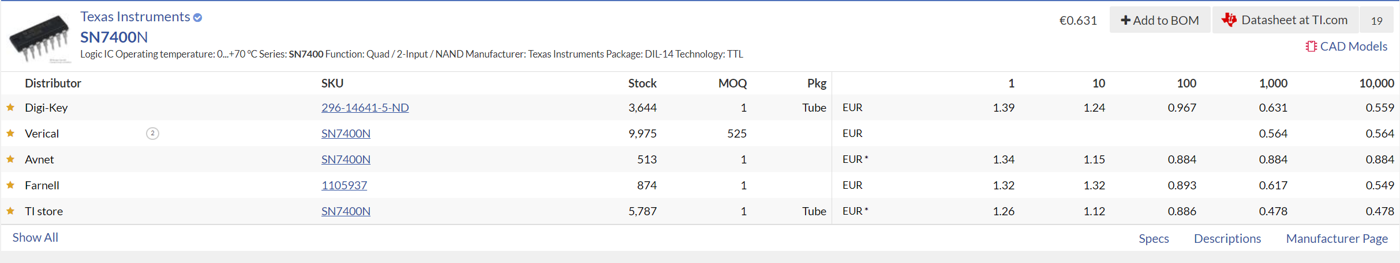
\includegraphics[width=9cm]{images/sn7400}
\end{textblock*}
\vspace{1cm}
\begin{columns}[b]
\begin{column}{0.5\textwidth}
\begin{itemize}
\item Real-World Problem
\begin{itemize}
\item Which suppliers to select to provide list of components
\item Limit number of suppliers by ordering multiple items from same supplier
\item Price/lead time/quality of service are competing objectives
\end{itemize}
\item Status
\begin{itemize}
\item Work with industry partner
\item Paper in Annals of Operations Research
\end{itemize}
\end{itemize}
\end{column}
\begin{column}{0.5\textwidth}
\begin{itemize}
\item Research Challenges
\begin{itemize}
\item How do we learn which choices are preferred
\item Difficult to assign fixed weights to different aspects of solution quality
\item Iterative, interactive learning of preferences
\end{itemize}
\item Solution Approach
\begin{itemize}
\item Preference Learning
\item Optimization
\end{itemize}
\end{itemize}
\end{column}
\end{columns}
\end{frame}

\begin{frame}
\frametitle{Optimizing UCC's CHP Plant Operation}
\begin{textblock*}{3.5cm}(10cm,-1cm)
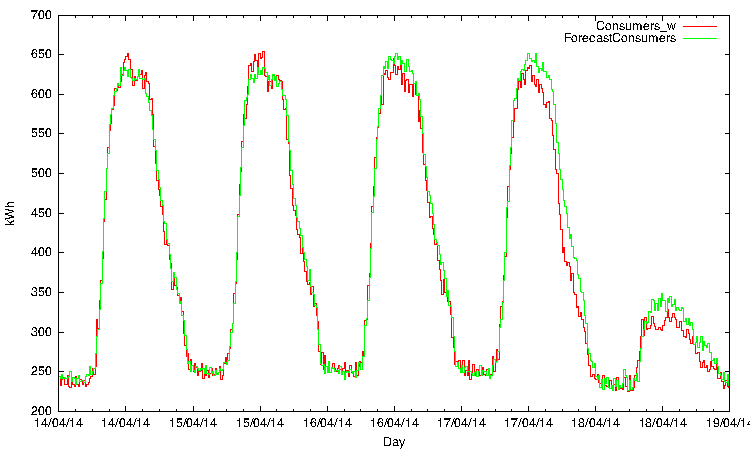
\includegraphics[width=3.5cm]{images/campusdemand}
\end{textblock*}
\vspace{0.5cm}
\begin{columns}[b]
\begin{column}{0.5\textwidth}
\begin{itemize}
\item Real-World Problem
\begin{itemize}
\item When to run UCC's CHP plant to create electricity/heat on-site
\item Needs demand forecast for heat and electricity
\item Uncertain Real-time grid electricity price
\item Heat and electricity demand of campus not in sync
\end{itemize}
\item Status
\begin{itemize}
\item Tested for several weeks with operator of plant
\item Part of EU Campus21 project
\end{itemize}
\end{itemize}
\end{column}
\begin{column}{0.5\textwidth}
\begin{itemize}
\item Research Challenges
\begin{itemize}
\item Heat and Electricity Demand prediction for campus
\item Price prediction for real-time grid price
\item Integration of plant operational constraints
\item Wider impact of heating strategy on campus 
\end{itemize}
\item Solution Approach
\begin{itemize}
\item Machine Learning
\item Optimization
\end{itemize}
\end{itemize}
\end{column}
\end{columns}
\end{frame}

\begin{frame}
\frametitle{CP Conference Paper Assignment Tool}
\begin{textblock*}{4cm}(10cm,-1cm)

\includegraphics[width=4cm]{images/cp2020logo}
\end{textblock*}
\begin{textblock*}{3cm}(10cm,0.5cm)

\includegraphics[width=3cm]{images/cp2021logo}
\end{textblock*}
\begin{columns}[b]
\begin{column}{0.5\textwidth}
\begin{itemize}
\item Real-World Problem
\begin{itemize}
\item Which reviewers to assign to papers 
\item Consider bids by reviewers, avoid assigning unwanted papers
\item Deal with reviewers shared between multiple tracks 
\item Balance assignment between reviewers
\item Allow pre-assignment, specific capacity constraints
\end{itemize}
\item Status
\begin{itemize}
\item Joint work with Data61, INRA
\item Used in 2020, 2021
\item Paper at ModRef 2020
\end{itemize}
\end{itemize}
\end{column}
\begin{column}{0.5\textwidth}
\begin{itemize}
\item Research Challenges
\begin{itemize}
\item Fair treatment of papers and reviewers
\item Finding mechanisms to allow Program Chair to control process
\item Not a black-box assignment
\item Integration with easychair
\end{itemize}
\item Solution Approach
\begin{itemize}
\item Optimization
\end{itemize}
\end{itemize}
\end{column}
\end{columns}
\end{frame}

}

\part{Success Stories}
\frame{\partpage}

\mode<all>{\begin{frame}
\frametitle{Success Stories}
\begin{itemize}
\item Some examples which show impact of CP
\item Not just a nice model or a novel constraint
\item Impact of solution
\item Recognition of CP as best tool for the job
\end{itemize}
\end{frame}

\section{Rosetta/Philae Mission Scheduling, LAAS-CNRS}

\begin{frame}
\frametitle{Scheduling of Data Transfer on Philae Lander}
\begin{columns}
\begin{column}{0.5\textwidth}
\begin{itemize}
\item Rosetta/Philae Mission 2004-2014
\item Land on a comet
\item Perform experiments
\item How do the data get back to earth?
\end{itemize}
\end{column}
\begin{column}{0.5\textwidth}
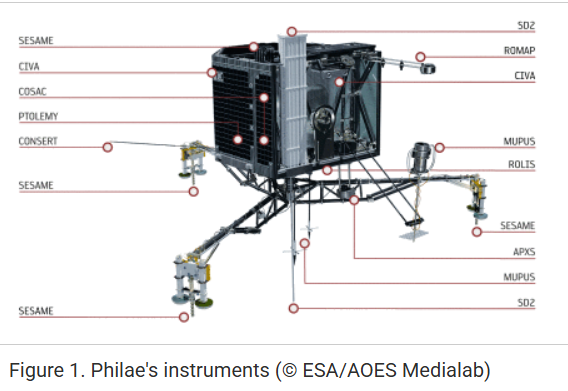
\includegraphics[width=\textwidth]{../summerschool2026/images/philae}
\end{column}
\end{columns}
\end{frame}

\begin{frame}
\frametitle{CP on a Comet?}
\begin{itemize}
\item Constraint model schedules data transfers between Rosetta (orbiter) and Philae (lander)
\item Part of the software suite controlling the lander
\item Developed by LAAS-CNRS, Toulouse
\begin{itemize}
\item Running on earth, not in the lander!
\end{itemize}
\item Written in Ilog Scheduler
\item To learn more: Simonin et al, 2015: Scheduling scientific experiments for comet exploration
\item Also: ACP Website \url{https://www.a4cp.org/node/1058}
\end{itemize}
\end{frame}

\begin{frame}
\frametitle{Global Constraint Model}
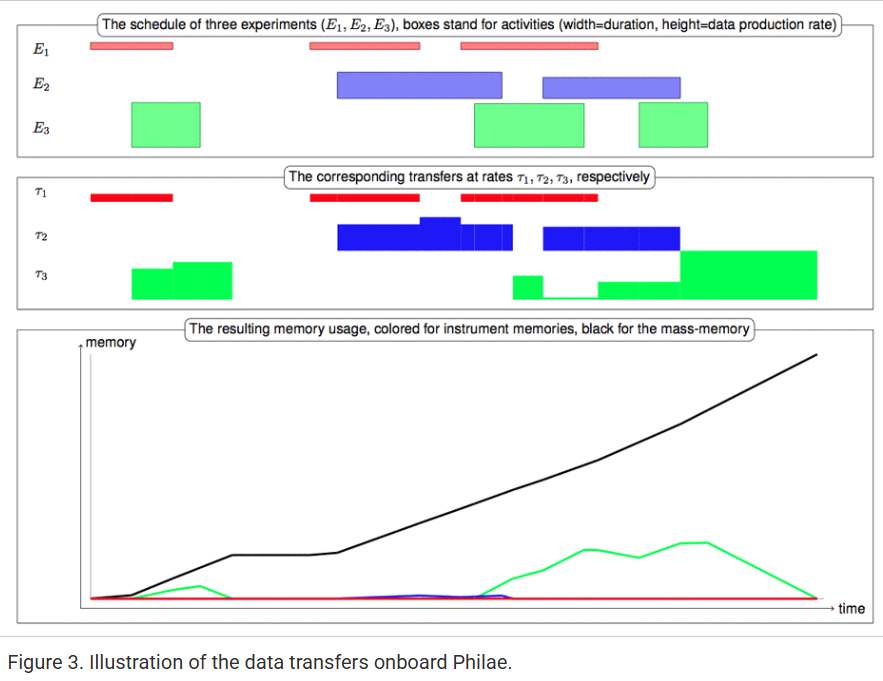
\includegraphics[width=9cm]{../summerschool2026/images/philaedatatransfer}
\end{frame}

\begin{frame}
\frametitle{Rosetta/Philae in popular culture}
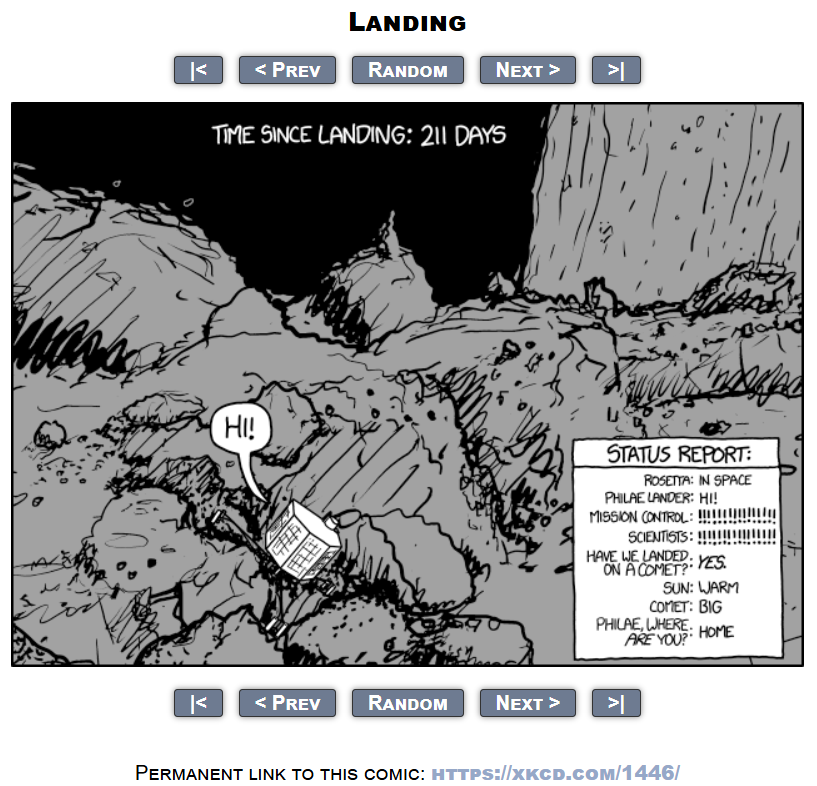
\includegraphics[width=7cm]{images/xkcd1446}
\end{frame}

\section{Unison Compiler, SICS, KTH, Ericsson, 2010-2018}

\begin{frame}
\frametitle{Unison}
\begin{itemize}
\item Long-term project to develop CP Based optimising compiler
\begin{itemize}
\item Instruction selection
\item Register allocation
\item Instruction scheduling
\end{itemize}
\item Integrates in \href{http://llvm.org}{LLVM} toolchain
\item Targeted for embedded systems processors
\end{itemize}
\end{frame}

\begin{frame}
\frametitle{What is the problem?}
\begin{itemize}
\item Translate high-level language into assembly code
\item Map variables to registers and memory
\item Map statements to instruction sequences
\item Modern processors are powerful, but complicated!
\item Complex resource allocation and scheduling problem
\item Most compact/ most performant code?
\item Must work all the time
\item Improvements are shared by all users (huge impact)
\end{itemize}
\end{frame}

\begin{frame}
\frametitle{Example High-level Program}
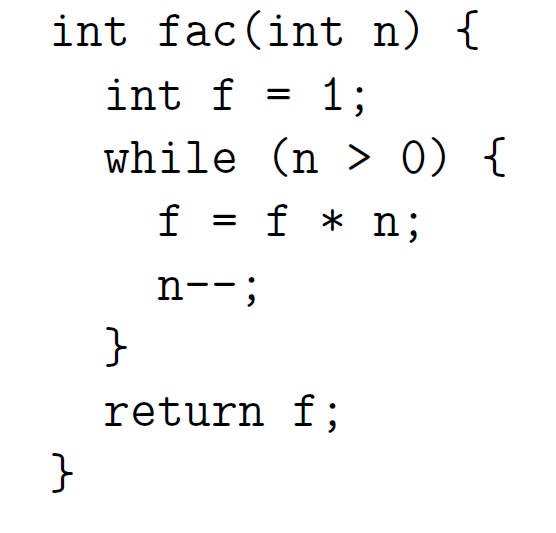
\includegraphics[width=6cm]{../summerschool2026/images/unisonexample}

\end{frame}

\begin{frame}
\frametitle{Generated Code Comparison (subtle)}
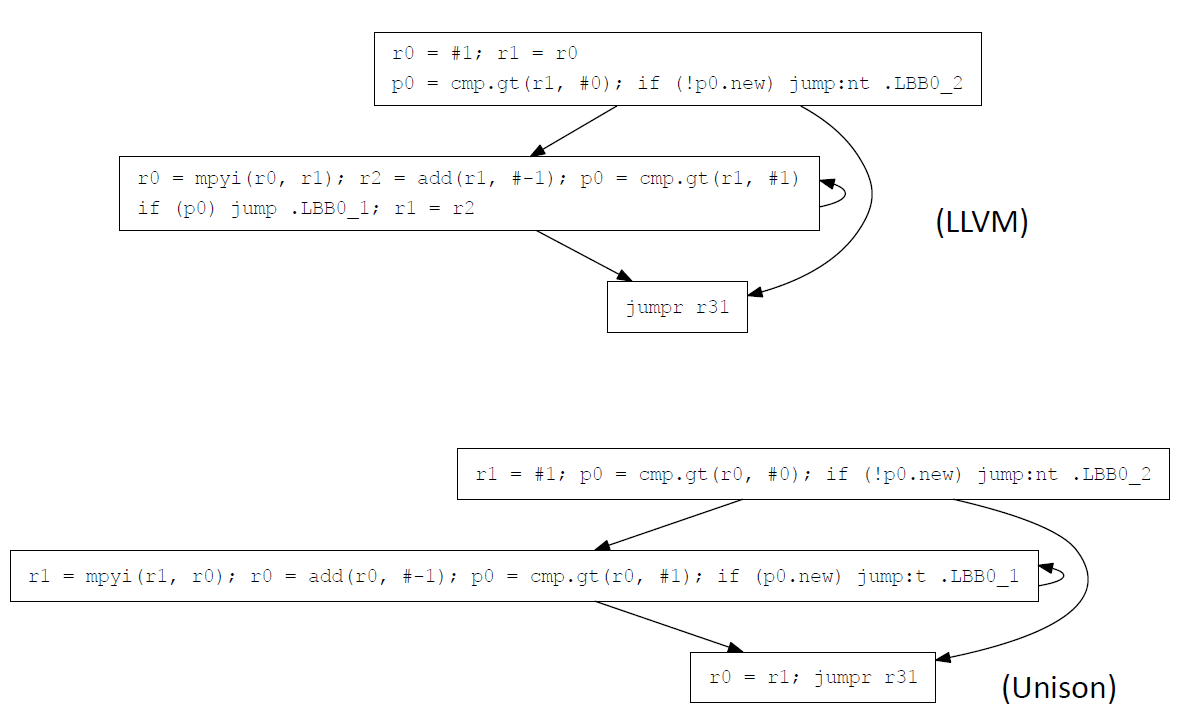
\includegraphics[width=10cm]{../summerschool2026/images/unisoncode}
\end{frame}

\begin{frame}
\frametitle{Unison Speedup Compared to LLVM}
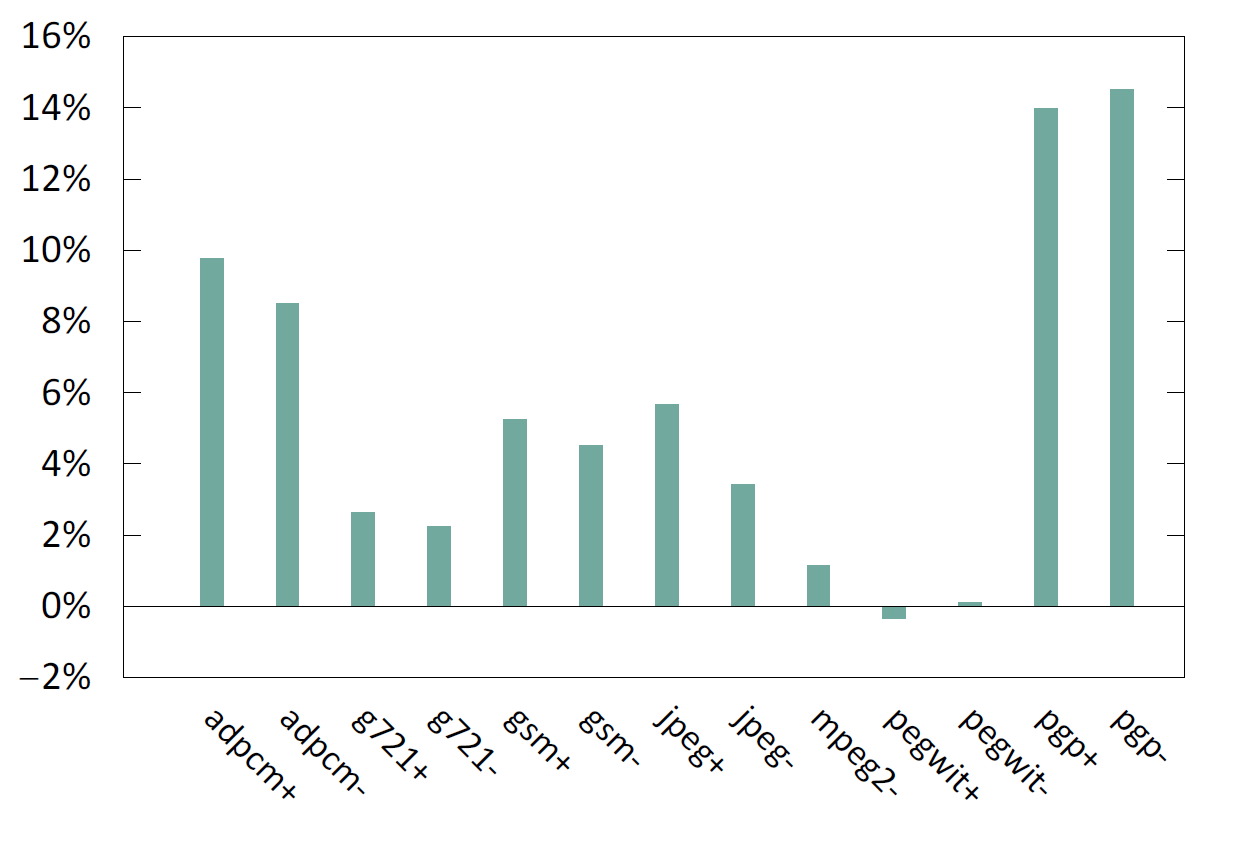
\includegraphics[width=10cm]{../summerschool2026/images/unisonspeedup}
\end{frame}

\begin{frame}
\frametitle{Conclusions}
\begin{itemize}
\item State-of-the-art compiler
\item Multiplier effect of improvements, everybody wins!
\item Significant number of publications outside CP domain
\item To learn more: Roberto Castaneda Lozano, NordConsNet 2025: Working in Unison with Mats \url{https://pierre-flener.github.io/research/NordConsNet/NordConsNet25/}
\end{itemize}
\end{frame}


%\section{Molecular Design, Thomas Schiex CP 2023}

%\section{Workforce Rostering, IBM Haifa, CP 2011}
}

\part{Methodology}
\frame{\partpage}

\mode<all>{\input{../summerschool2026/methodology}}

\part{Additional Resources}
\frame{\partpage}

\mode<all>{\section{Tools}

\begin{frame}
\frametitle{Tools already discussed in Summer School}
\begin{itemize}
\item \href{https://minizinc.org}{MiniZinc}
\item \href{https://cpmpy.readthedocs.io}{CPMpy}
\item \href{https://github.com/ciaranm/glasgow-constraint-solver}{Glasgow Constraint Solver}
\end{itemize}
\end{frame}

\begin{frame}
\frametitle{Other Academic Solvers}
\begin{itemize}
\item Gecode (KTH, Sweden)
\item Choco-solver (IMT Atlantique, France)
\item MiniCP (Louvain, U Conn, Georgia Tech)
\item MaxiCP (Louvain, U Conn, Georgia Tech)
\item SICStus Prolog (RISE, Sweden) 
\end{itemize}
\end{frame}

\begin{frame}
\frametitle{Commercial Tools}
\begin{itemize}
\item \href{https://ibm.com}{CP Optimizer}
\begin{itemize}
\item P. Laborie et al, 2018: IBM ILOG CP optimizer for scheduling
20+ years of scheduling with constraints at IBM/ILOG
\end{itemize}

\item \href{https://developers.google.com}{CP-Sat}
\begin{itemize}
\item L. Perron et al, Invited Talk, CP 2023: The CP-SAT-LP Solver
\item \href{https://www.youtube.com/embed/vvUxusrUcpU?si=ldUAKR6WqdfAIrhL}{Video in Scheduling Seminar}
\end{itemize}

\item \href{https://optalcp.com}{OptalCP}
\begin{itemize}
\item P. Vilim, Invited Talk, CP 2023: CP Solver Design for Maximum CPU Utilization
\item \href{https://www.youtube.com/embed/1Dm-kY3ekKo?si=wn34td-NrpOxknB4}{Video in Scheduling Seminar}
\end{itemize}

\item \href{https://hexaly.com}{Hexaly}
\begin{itemize}
\item T. Benoist, Tutorial at CP 2026
\item \href{https://www.youtube.com/embed/VjB5FoaFFUM?si=27yxZJAfkEBroxZf}{Video in Scheduling Seminar}
\end{itemize}
\end{itemize}
\end{frame}

\section{Learning Materials}

\begin{frame}
\frametitle{Learning Materials}
\begin{itemize}
\item Workshops on Teaching CP at CP 2015, CP 2023 \url{https://hsimonis.github.io/WTCP2023/index.html}
\item Survey of teaching materials with Tejas Santanam (Georgia Tech)
\item Available at \url{https://arxiv.org/abs/2403.12717}
\end{itemize}
\end{frame}

\section{Companies}

\begin{frame}
\frametitle{IBM and Constraint Programming}
\begin{quote}
Constraint programming technology is used to find solutions to scheduling and combinatorial optimization problems. It is based primarily on computer science fundamentals, such as logic programming and graph theory, in contrast to mathematical programming, which is based on numerical linear algebra.

Constraint programming is invaluable when dealing with the complexity of many real-world sequencing and scheduling problems.
\end{quote}
IBM {\tiny (\url{https://ibmdecisionoptimization.github.io/docplex-doc/cp.html})}
\end{frame}

\begin{frame}
\frametitle{Examples}
\begin{itemize}
\item Cosling, France
\item OptalCP, France, Czech Republic
\item Hexaly, France
\item Keelvar, Ireland
\item Opturion, Australia
\item Optix Solutions, Hong Kong
\end{itemize}
\end{frame}

\begin{frame}
\frametitle{\href{https://www.cosling.com}{Cosling}}
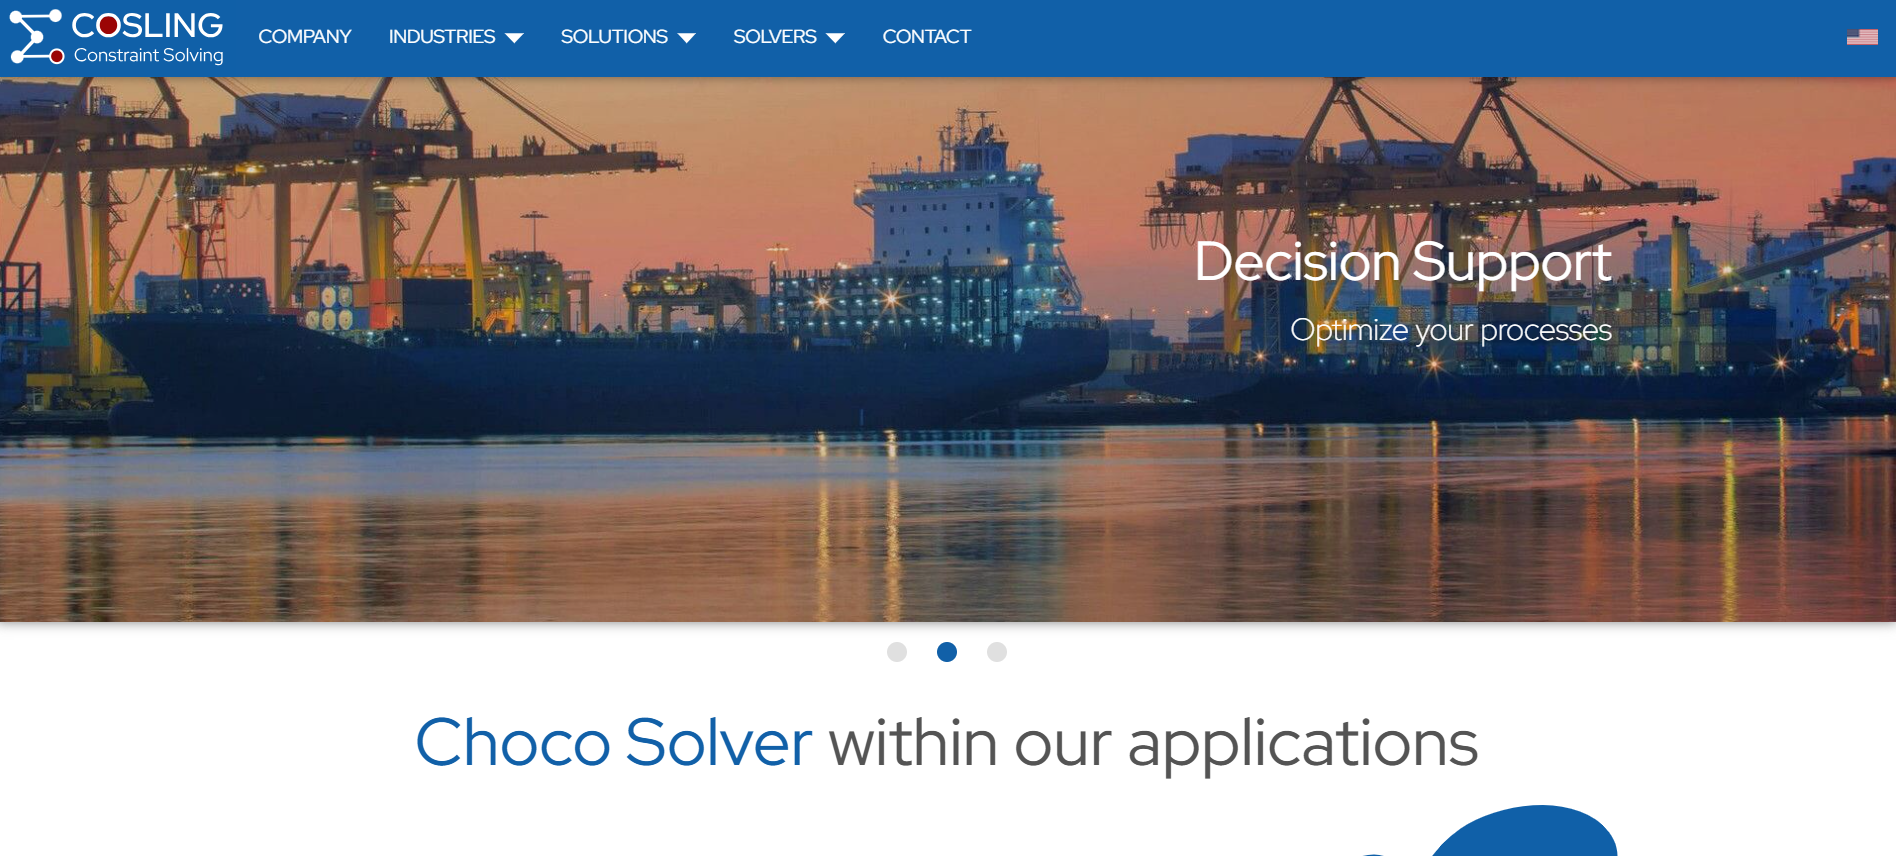
\includegraphics[width=12cm]{images/cosling.png}
\end{frame}

\begin{frame}
\frametitle{\href{https://www.optalcp.com}{OptalCP}}
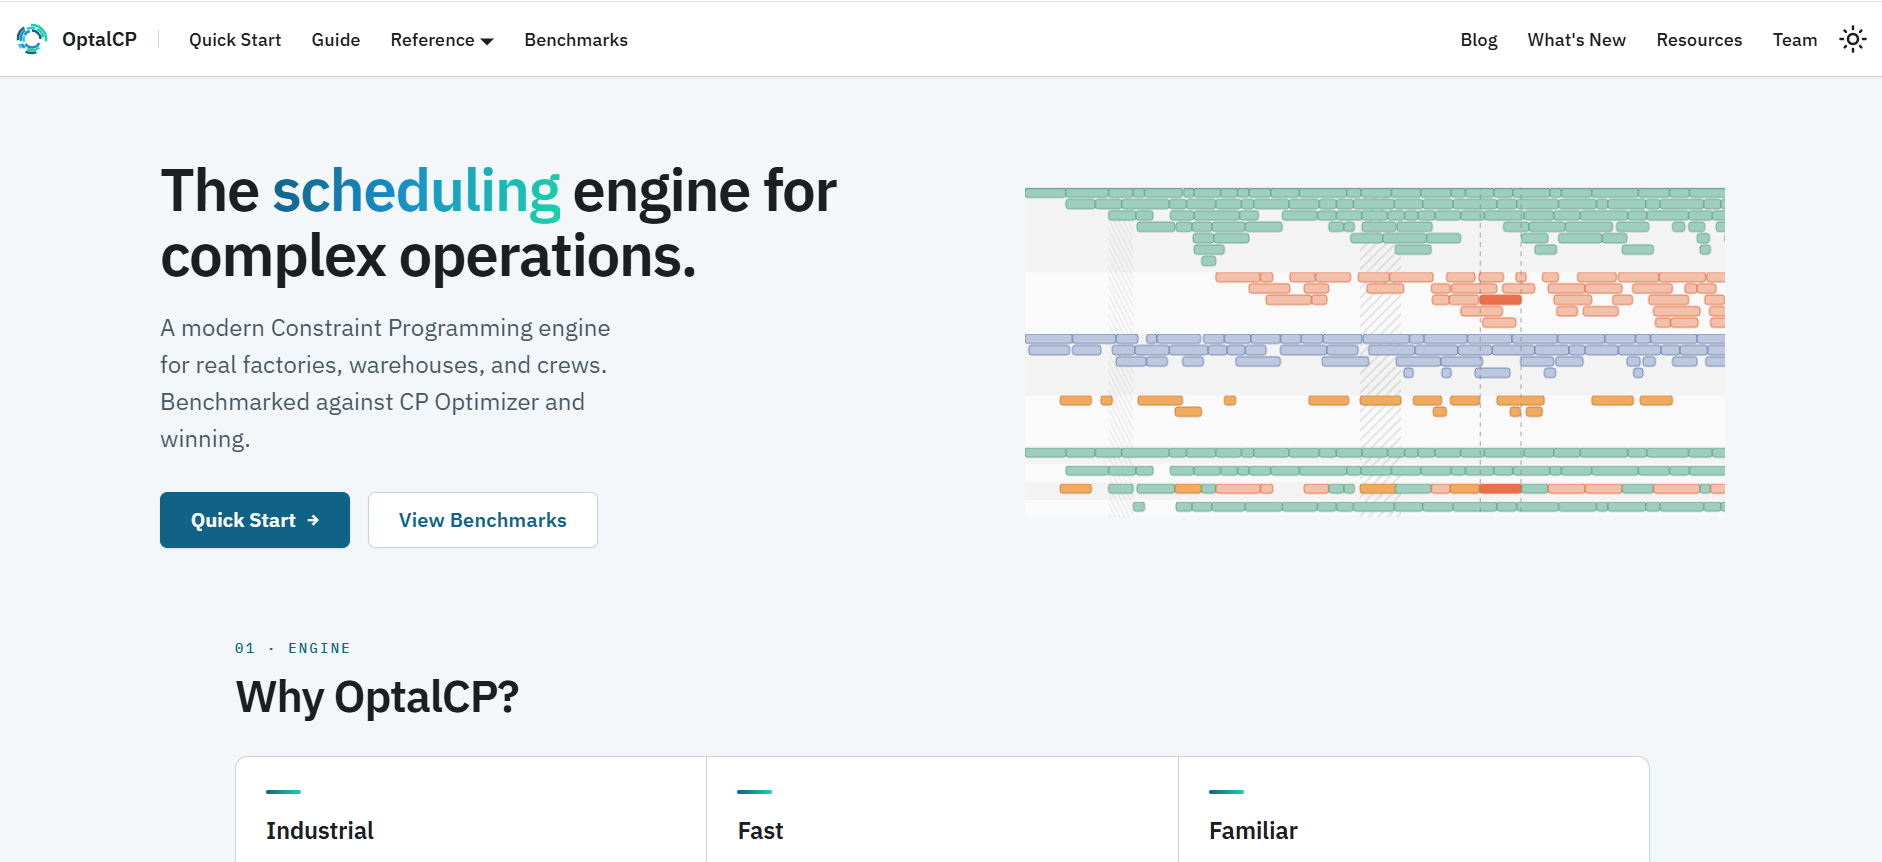
\includegraphics[width=12cm]{images/optalcp.png}
\end{frame}

\begin{frame}
\frametitle{\href{https://www.hexaly.com}{Hexaly}}
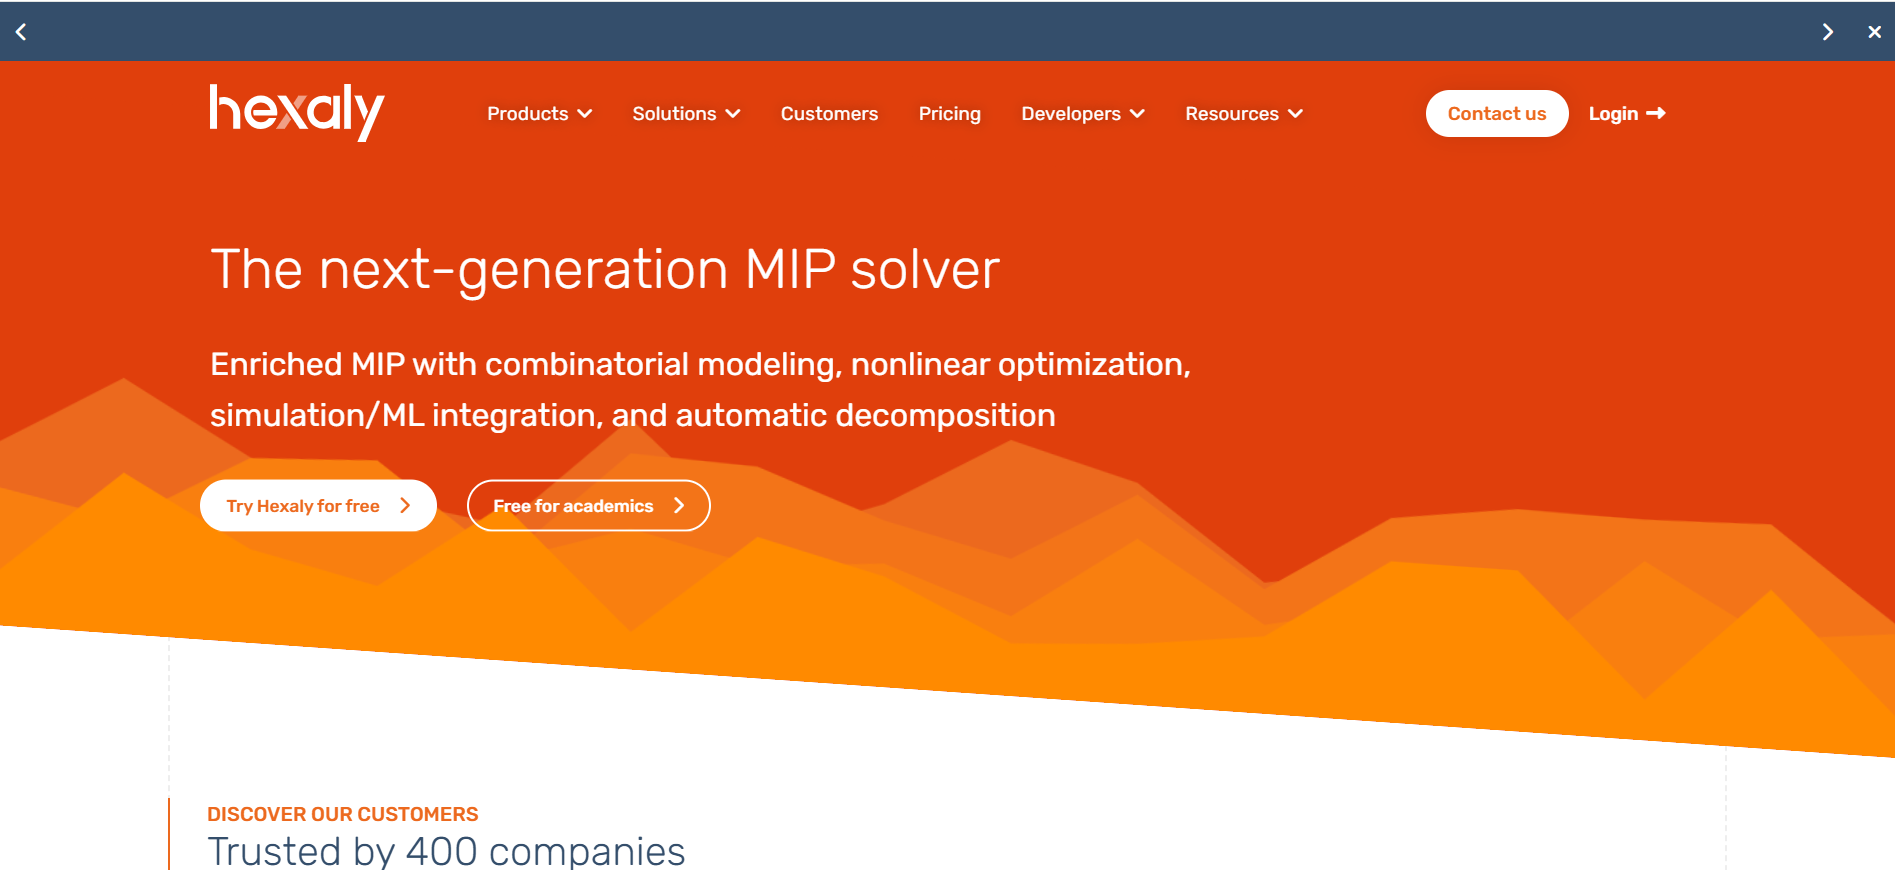
\includegraphics[width=12cm]{images/hexaly.png}
\end{frame}

\begin{frame}
\frametitle{\href{https://www.keelvar.com}{Keelvar}}
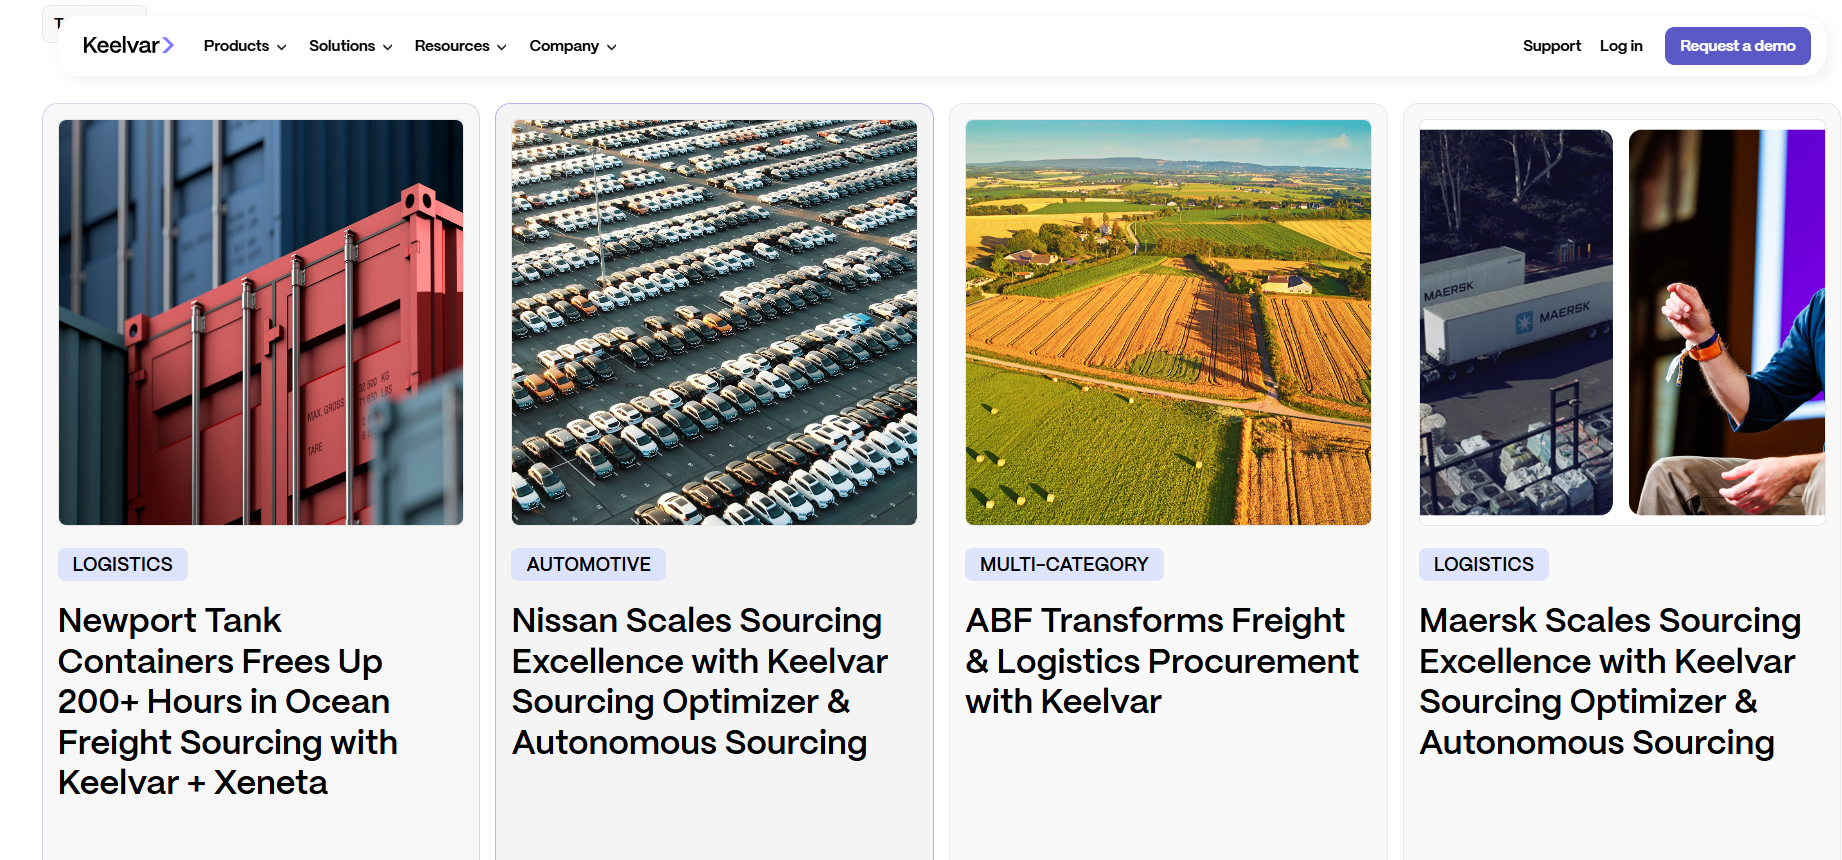
\includegraphics[width=12cm]{images/keelvar.png}
\end{frame}

\begin{frame}
\frametitle{\href{https://www.opturion.com}{Opturion}}
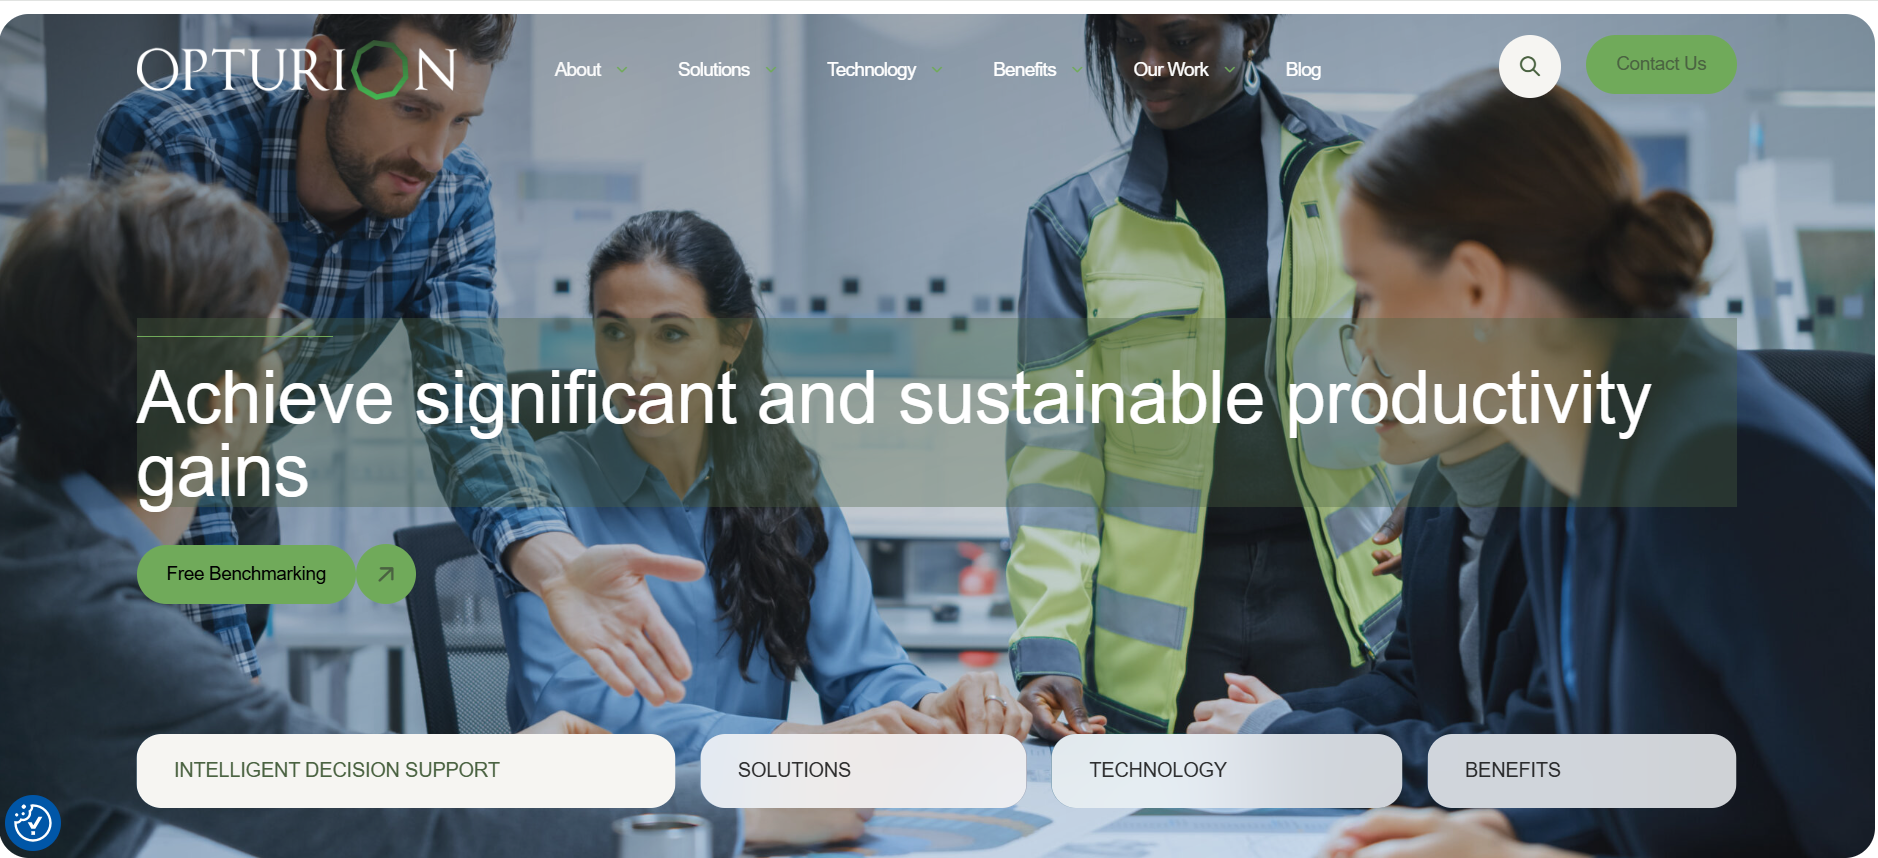
\includegraphics[width=12cm]{images/opturion.png}
\end{frame}

\begin{frame}
\frametitle{\href{https://www.optixsolutions.com.hk}{Optix Solutions}}

\includegraphics[width=12cm]{images/optixsolutions.png}
\end{frame}

\section{Literature Overview}

\begin{frame}
\frametitle{Literature Overview}
\begin{itemize}
\item Getting started in field can be overwhelming
\item A lot of work has been done
\item What is most relevant?
\item What is most related to what I want to do?
\item Where should I publish?
\item Getting to know the community
\end{itemize}
\end{frame}

\subsection{CP Conference}

\begin{frame}
\frametitle{CP Conference}
\begin{itemize}
\item Organised by Association for Constraint Programming (ACP)
\item Yearly since 1995
\item Special application track since 2002
\item CP 2027 will be here in Jilin
\item Survey of all papers since 2010 
\item Online version at \url{https://hsimonis.github.io/pthg24/cpconference.pdf}
\end{itemize}
\end{frame}

\begin{frame}
\frametitle{CP Conference Papers by Track}
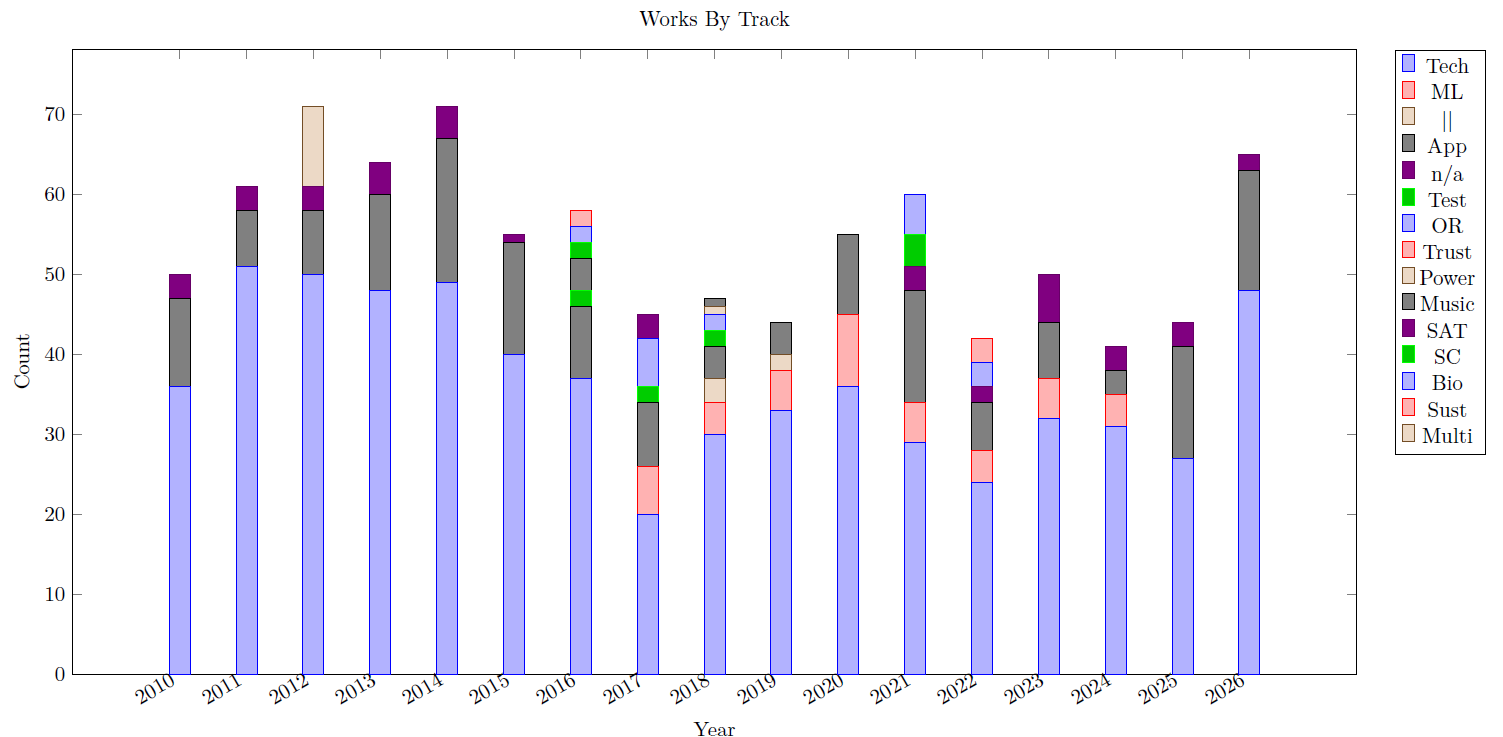
\includegraphics[width=12cm]{images/cpbytrack}
\end{frame}

\begin{frame}
\frametitle{CP Conference Award Winning Papers}
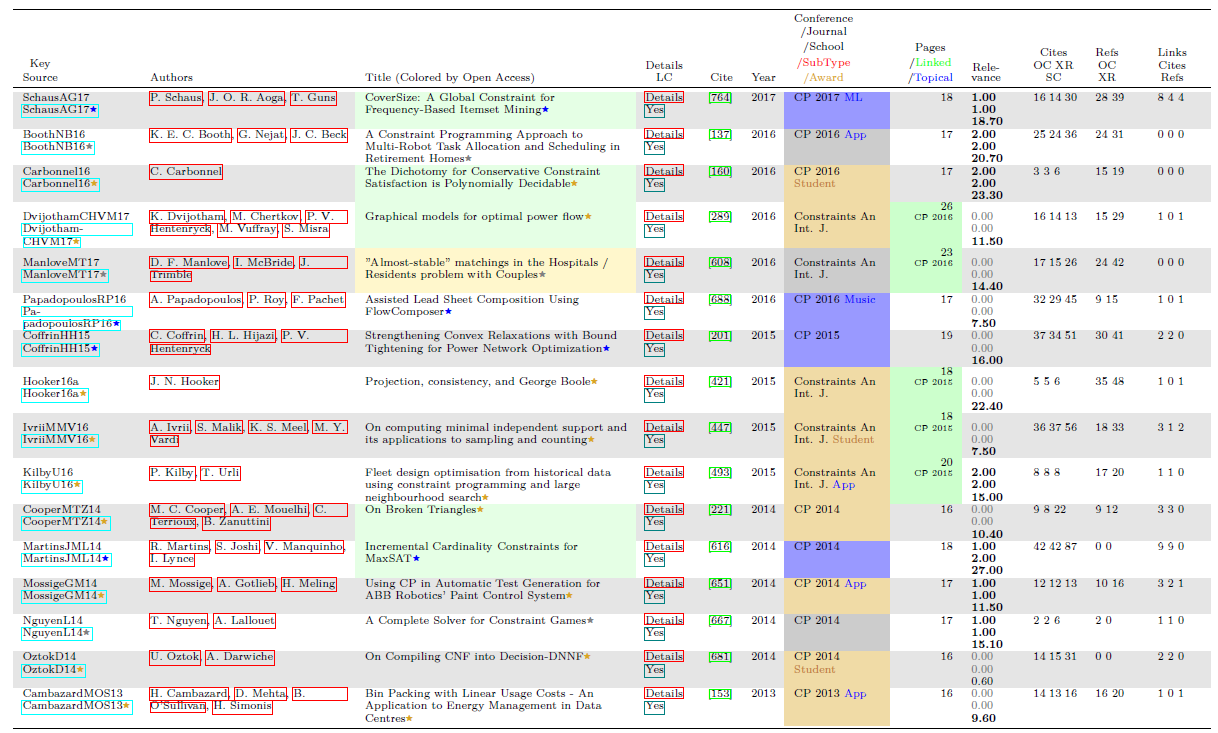
\includegraphics[width=12cm]{images/cpawardwinning}
\end{frame}

\begin{frame}
\frametitle{CP Conference Most Cited Papers}
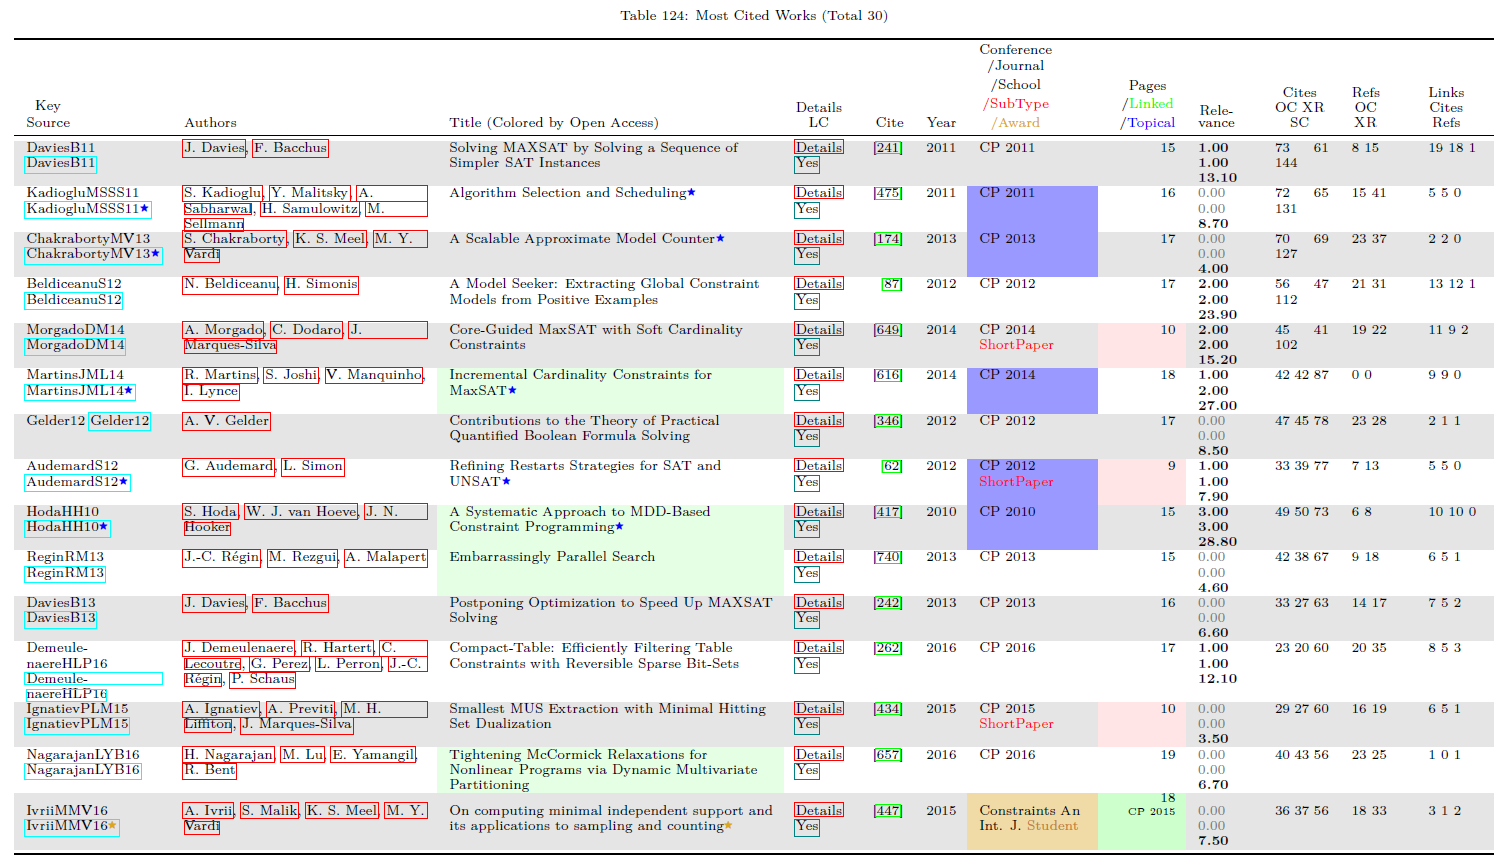
\includegraphics[width=12cm]{images/cpmostcited}
\end{frame}

\subsection{Constraints Journal}

\begin{frame}
\frametitle{Constraints Journal}
\begin{itemize}
\item Shameless plug by EiC (me)
\item Published by Springer
\item 30 years, started in 1996
\item Often publishes extended versions of CP/CPAIOR conference papers
\item Also longer form original articles
\item Submissions welcome!
\item Survey online version at \url{https://hsimonis.github.io/pthg24/constraints.pdf}
\item A data analysis at \url{https://hsimonis.github.io/pthg24/slidescp2026.pdf}
\end{itemize}
\end{frame}

\begin{frame}
\frametitle{Constraints Journal Articles by Country}
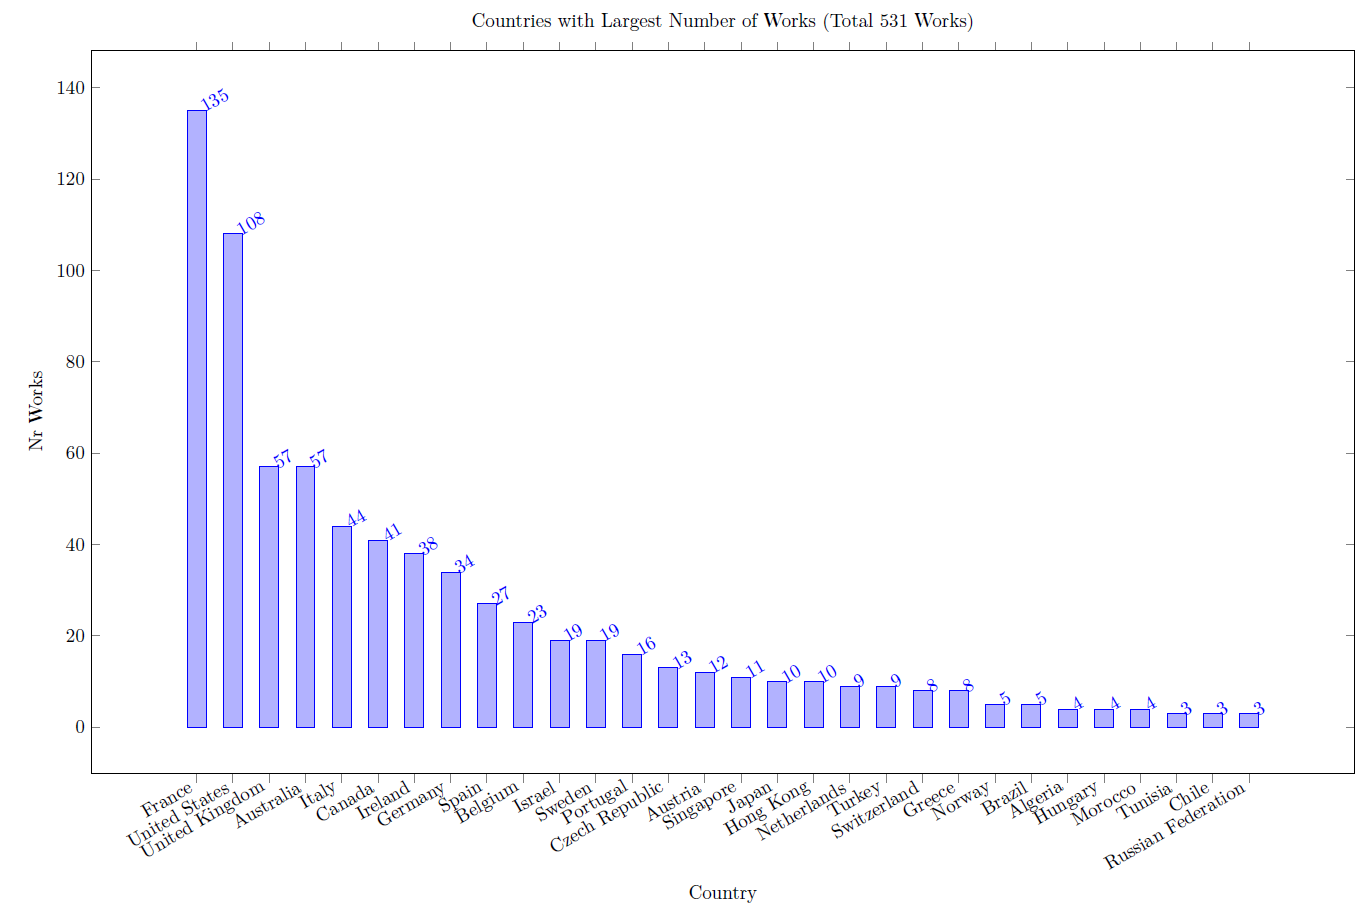
\includegraphics[width=11cm]{images/constraintscountry}
\end{frame}

\begin{frame}
\frametitle{Constraints Journal Citations}
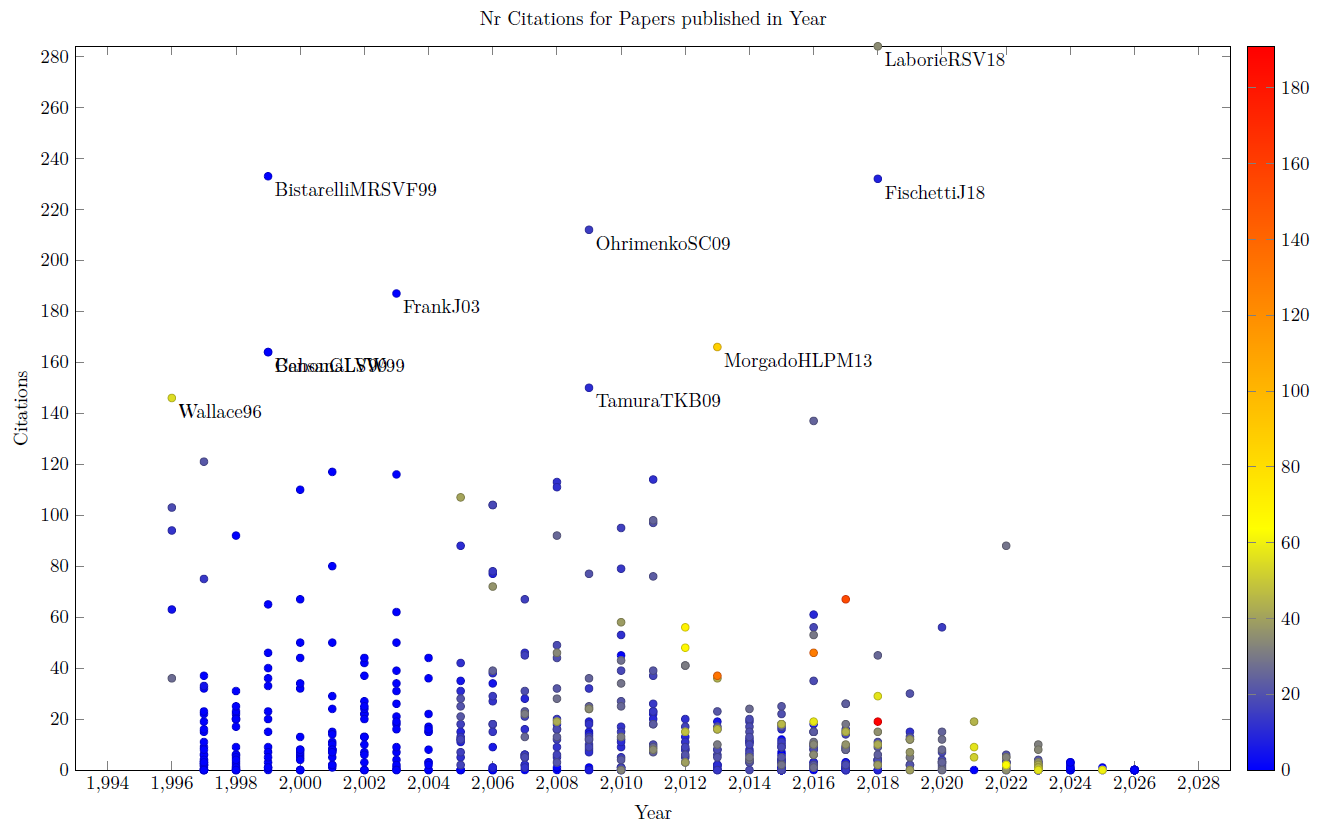
\includegraphics[width=11cm]{images/constraintscitations}
\end{frame}

\begin{frame}
\frametitle{Constraints Journal Special Issues}
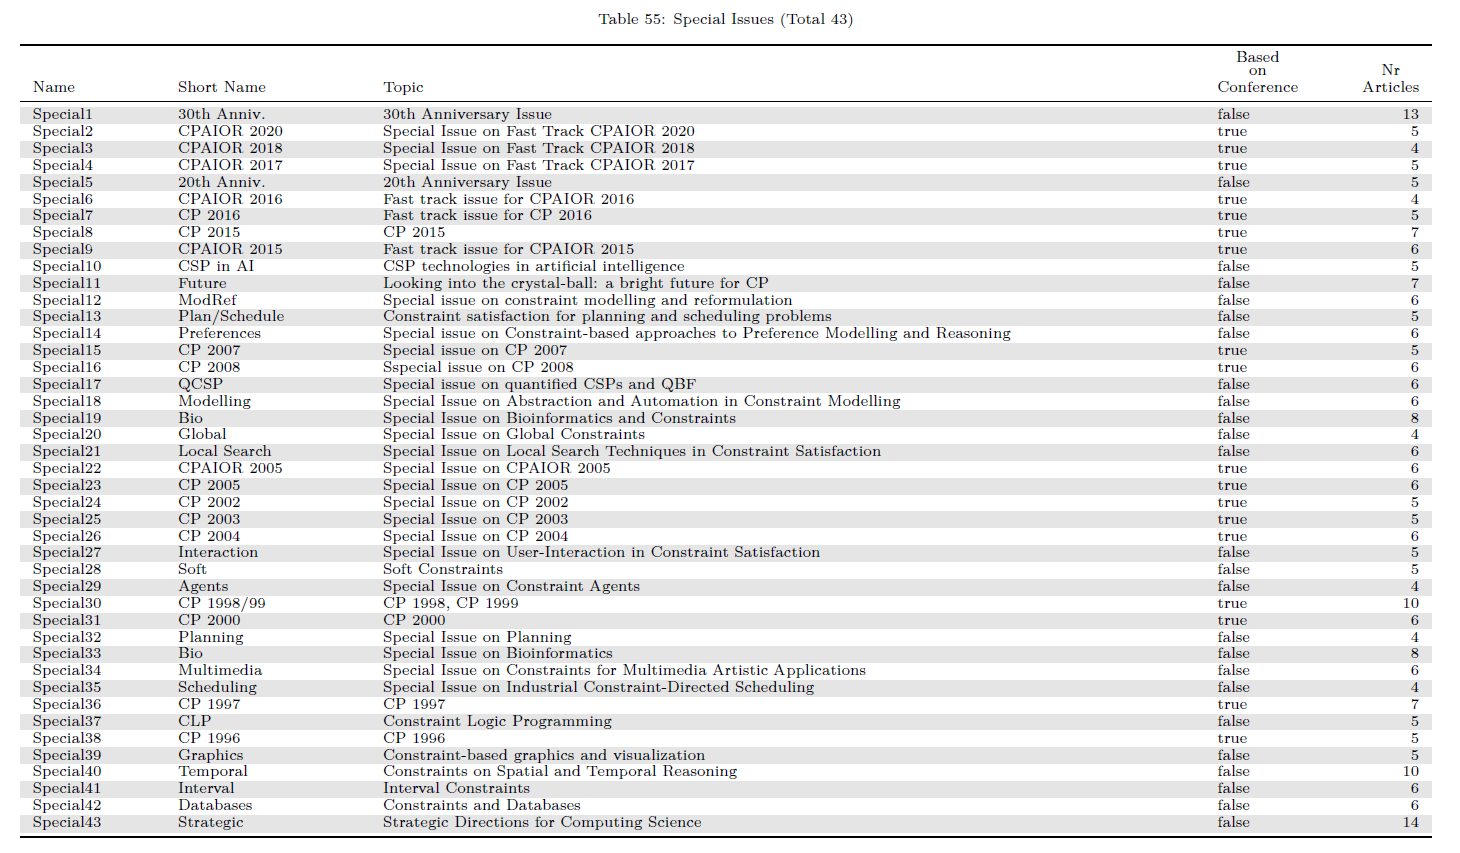
\includegraphics[width=12cm]{images/constraintsspecialissues}
\end{frame}



\subsection{CP and Scheduling}

\begin{frame}
\frametitle{}
\begin{itemize}
\item Joint work with Cemal Ozturk (MTU)
\item Overview of works combining CP with scheduling
\item Works since 1980
\item Survey online at \url{https://hsimonis.github.io/pthg24/scheduling.pdf}
\end{itemize}
\end{frame}

\begin{frame}
\frametitle{CP \& Scheduling Conferences}
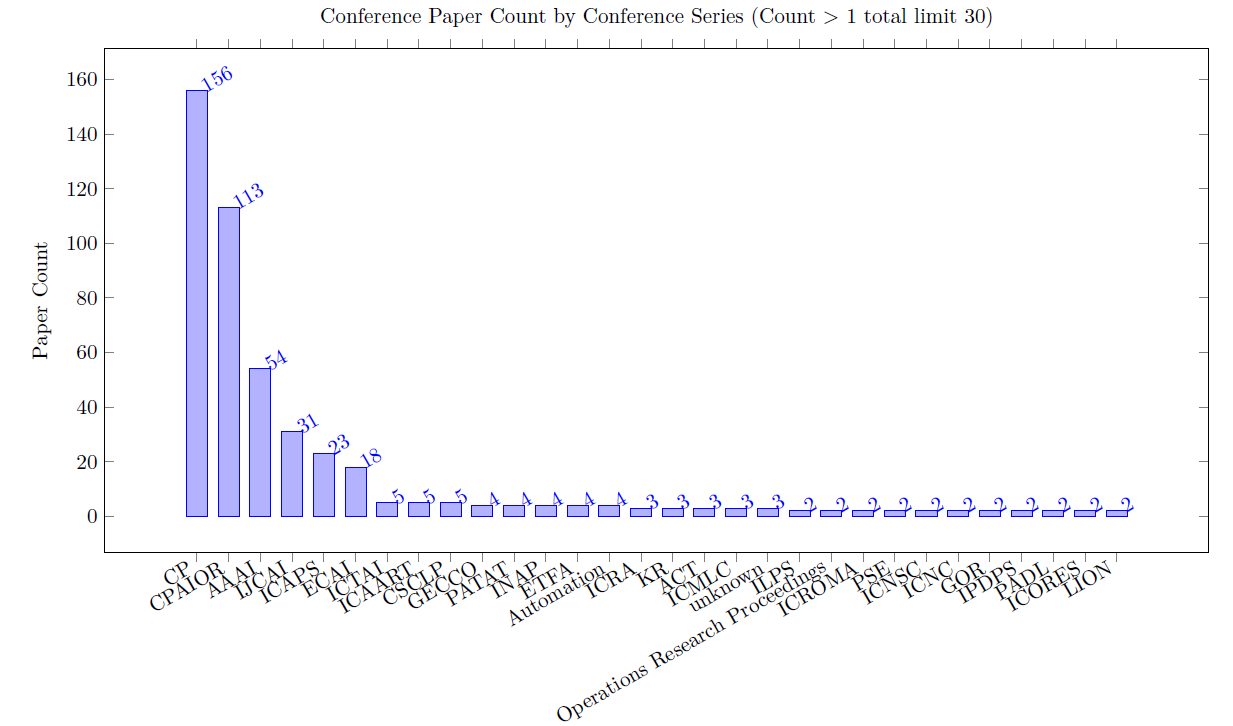
\includegraphics[width=12cm]{images/schedulingconferences}
\end{frame}

\begin{frame}
\frametitle{CP \& Scheduling Journals}
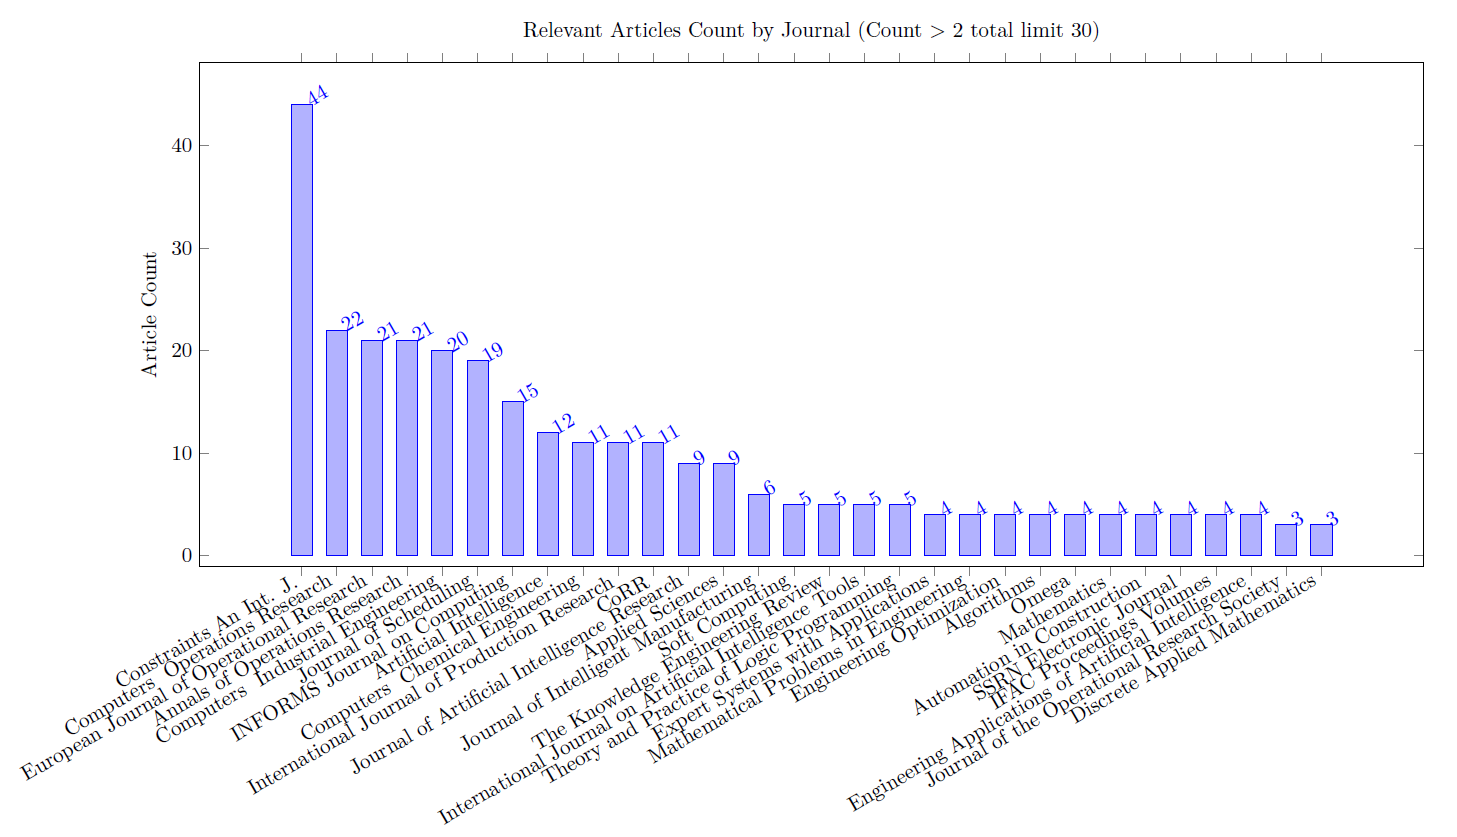
\includegraphics[width=12cm]{images/schedulingjournals}
\end{frame}

\begin{frame}
\frametitle{CP \& Scheduling Prolific Authors}
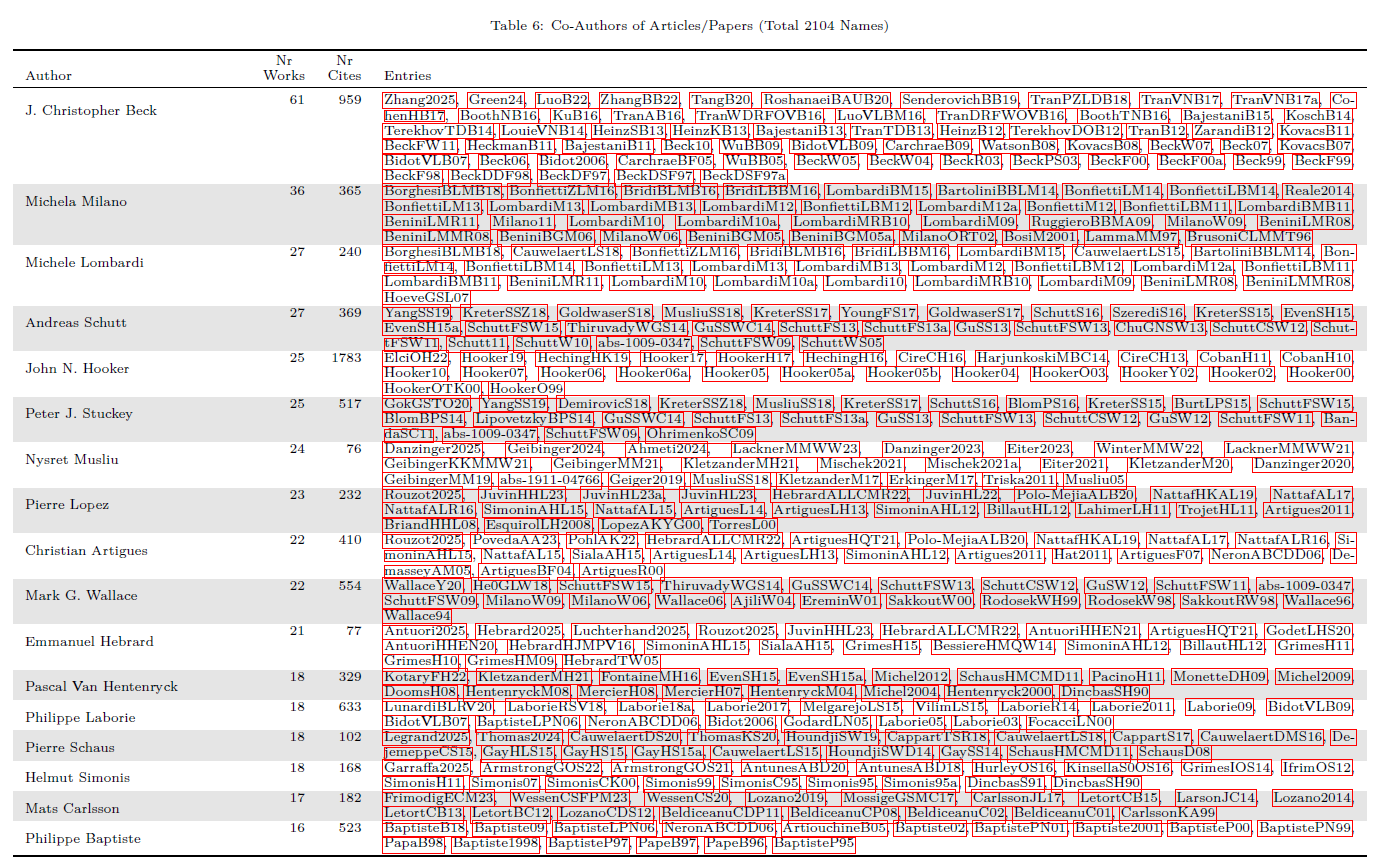
\includegraphics[width=11cm]{images/schedulingauthors}
\end{frame}

\begin{frame}
\frametitle{CP \& Scheduling Co-Author Graph (Excerpt)}
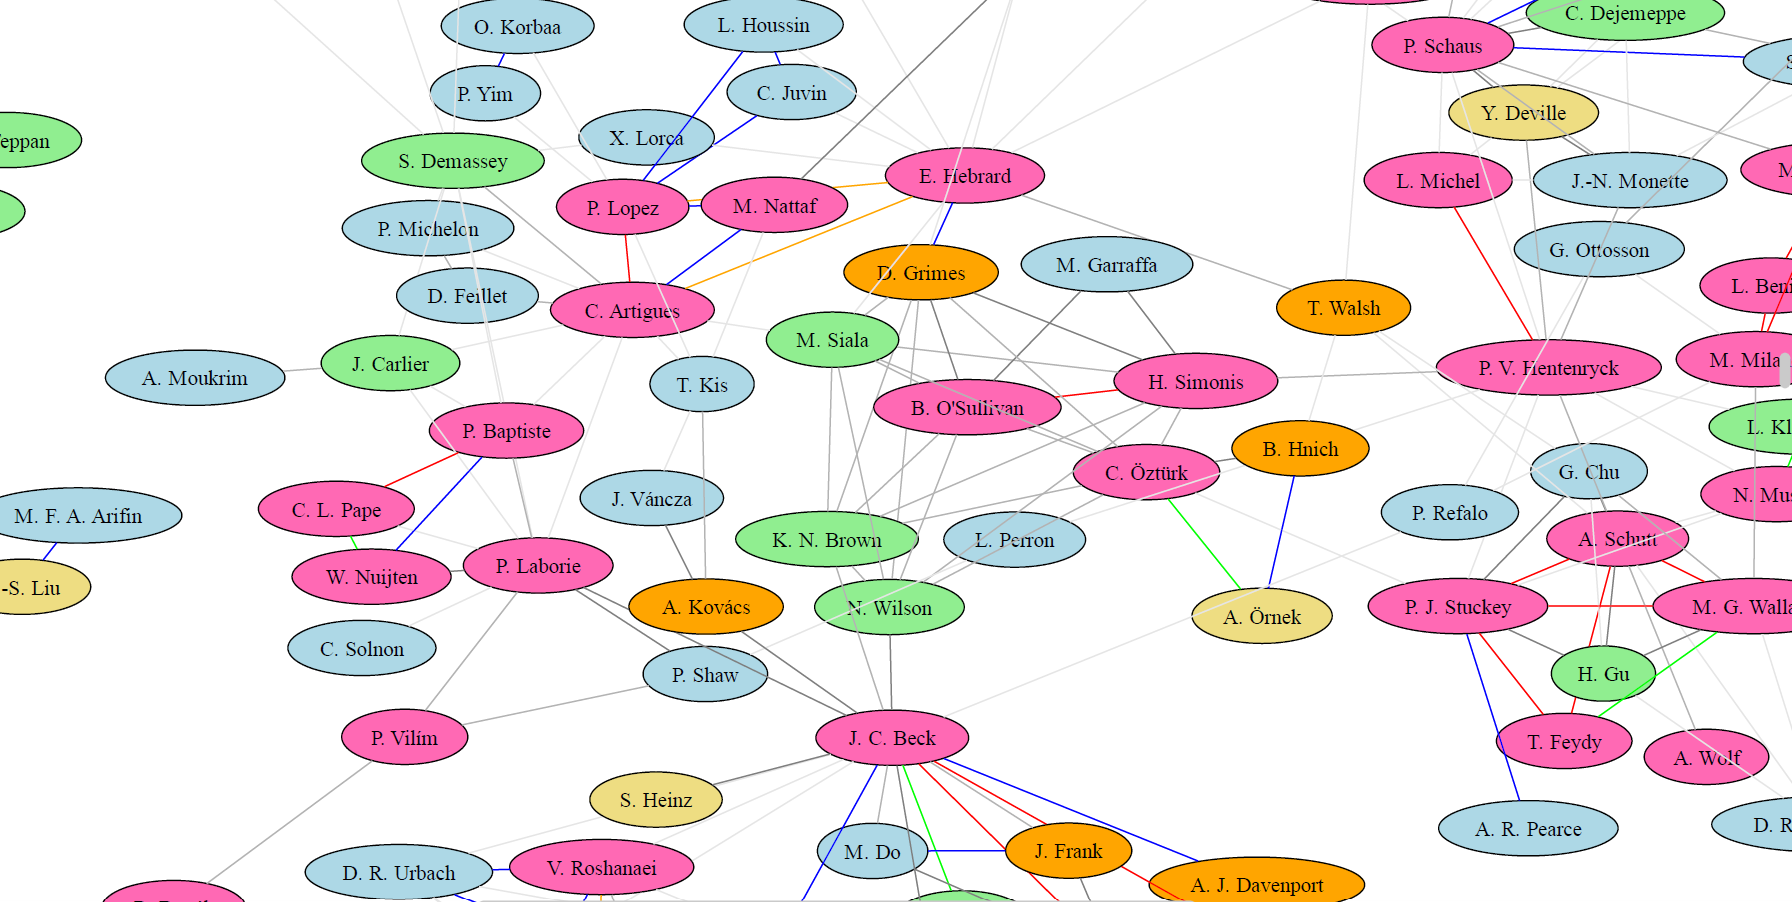
\includegraphics[width=11cm]{images/schedulingcoauthorgraph}
\end{frame}

\begin{frame}
\frametitle{CP \& Scheduling Concept Matching}
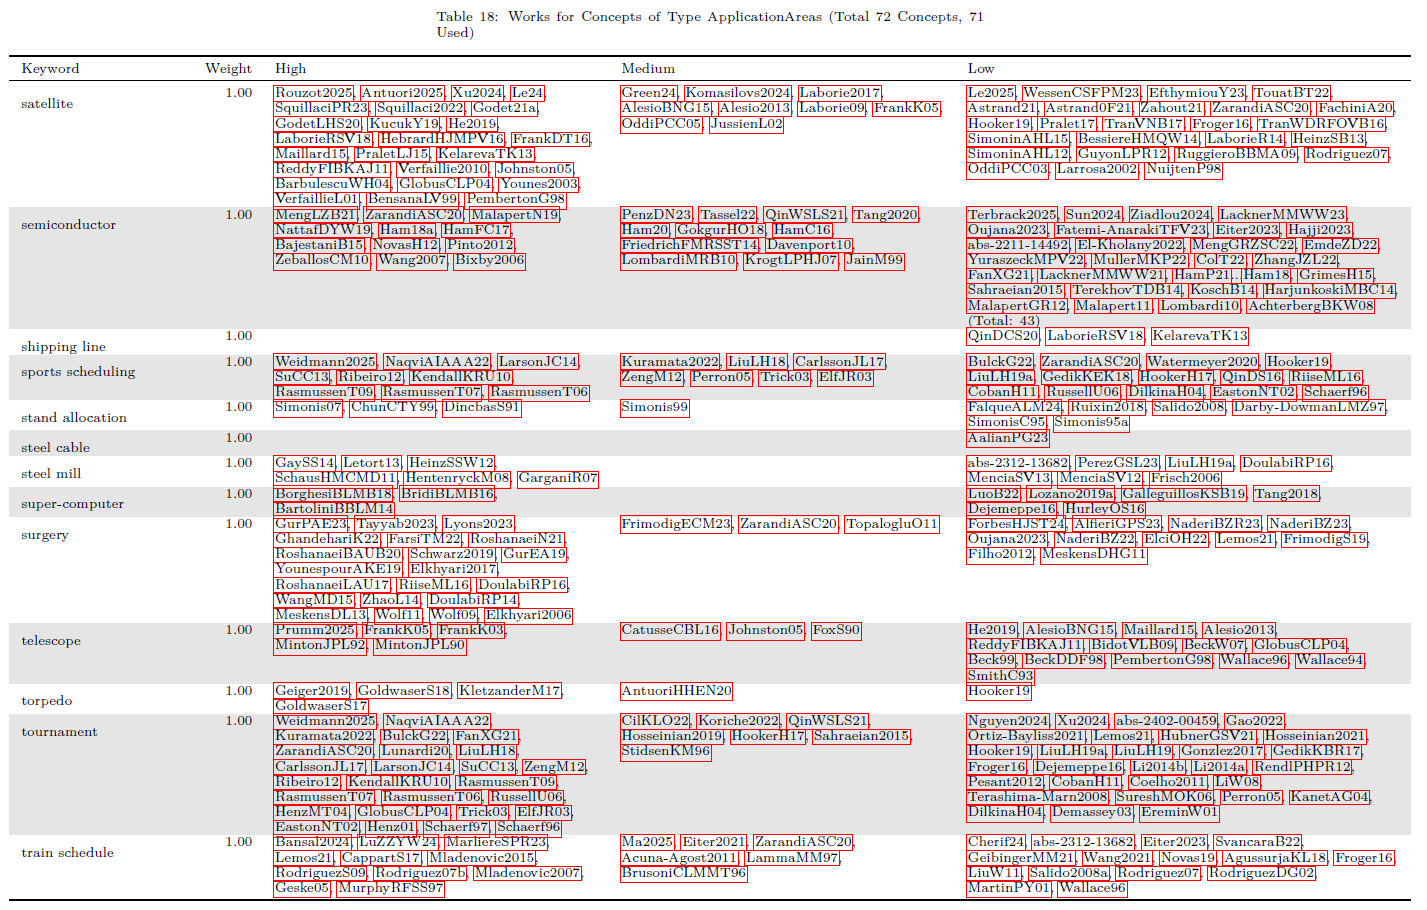
\includegraphics[width=12cm]{images/schedulingconcepts}
\end{frame}



}

\section{Summary}

\begin{frame}
\frametitle{Summary}
\begin{itemize}
\item Overview of applications and methodology
\item Highlights on success stories
\item Research can have a real impact
\item Your application could be next!
\item Provided details on some application work in Cork
\item Shows the impact of practical problems on basic research
\item It takes time to do application based research
\item Time well spent!
\end{itemize}
\end{frame}

